\documentclass[12pt]{article}
\usepackage{amsmath}
%\usepackage{graphicx,psfrag,epsf}
\RequirePackage{graphicx,color,ae,fancyvrb}

% \usepackage{psfrag,epsf}
\usepackage{enumerate}
\usepackage{natbib}
\usepackage{hyperref} % not crucial - just used below for the URL 


%\pdfminorversion=4
% NOTE: To produce blinded version, replace "0" with "1" below.
\newcommand{\blind}{0}

% DON'T change margins - should be 1 inch all around.
\addtolength{\oddsidemargin}{-.5in}%
\addtolength{\evensidemargin}{-.5in}%
\addtolength{\textwidth}{1in}%
\addtolength{\textheight}{1.3in}%
\addtolength{\topmargin}{-.8in}%

% Pandoc header
\usepackage{float}
\let\origfigure\figure
\let\endorigfigure\endfigure
\renewenvironment{figure}[1][2] {
    \expandafter\origfigure\expandafter[H]
} {
    \endorigfigure
}

\usepackage{amsmath} \usepackage{subfig} \usepackage{float} \renewcommand{\thesubfigure}{\Alph{subfigure}}

%% commands
%\newcommand\code{\bgroup\@makeother\_\@makeother\~\@makeother\$\@codex}
%\def\@codex#1{{\normalfont\ttfamily\hyphenchar\font=-1 #1}\egroup}
\let\code=\texttt

\let\proglang=\textsf
\newcommand{\pkg}[1]{{\fontseries{b}\selectfont #1}}

% \usepackage{color,ae,fancyvrb}

%% Sweave(-like)
\DefineVerbatimEnvironment{Sinput}{Verbatim}{fontshape=sl}
\DefineVerbatimEnvironment{Soutput}{Verbatim}{}
\DefineVerbatimEnvironment{Scode}{Verbatim}{fontshape=sl}
\newenvironment{Schunk}{}{}
\DefineVerbatimEnvironment{Code}{Verbatim}{}
\DefineVerbatimEnvironment{CodeInput}{Verbatim}{fontshape=sl}
\DefineVerbatimEnvironment{CodeOutput}{Verbatim}{}
\newenvironment{CodeChunk}{}{}
\setkeys{Gin}{width=0.8\textwidth}
%% footer

\newcommand\independent{\protect\mathpalette{\protect\independenT}{\perp}}
\def\independenT#1#2{\mathrel{\rlap{$#1#2$}\mkern2mu{#1#2}}}


\begin{document}

%\bibliographystyle{natbib}

\def\spacingset#1{\renewcommand{\baselinestretch}%
{#1}\small\normalsize} \spacingset{1}


%%%%%%%%%%%%%%%%%%%%%%%%%%%%%%%%%%%%%%%%%%%%%%%%%%%%%%%%%%%%%%%%%%%%%%%%%%%%%%

\if0\blind
{
  \title{\bf ROC and AUC with a Binary Predictor: a Potentially Misleading Metric} 
  \author{John Muschelli\thanks{This analysis was supported by NIH Grants R01NS060910 and U01NS080824 and Johns Hopkins Department of Biostatistics. }\hspace{.2cm}\\
	Department of Biostatistics, Johns Hopkins Bloomberg School of Public Health}
  \maketitle
} \fi

\if1\blind
{
  \bigskip
  \bigskip
  \bigskip
  \begin{center}
    {\LARGE\bf ROC and AUC with a Binary Predictor: a Potentially Misleading Metric}
\end{center}
  \medskip
} \fi

\bigskip
\begin{abstract}
In analysis of binary outcomes, the receiver operator characteristic
(ROC) curve is heavily used to show the performance of a model or
algorithm. The ROC curve is informative about the performance over a
series of thresholds and can be summarized by the area under the curve
(AUC), a single number. When a \textbf{predictor} is categorical, the
ROC curve has only as many thresholds as the one less than number of
categories; when the predictor is binary there is only one threshold. As
the AUC may be used in decision-making processes on determining the best
model, it important to discuss how it agrees with the intuition from the
ROC curve. We discuss how the interpolation of the curve between
thresholds with binary predictors can largely change the AUC. Overall,
we believe a linear interpolation from the ROC curve with binary
predictors, which is most commonly done in software, corresponding to
the estimated AUC. We believe these ROC curves and AUC can lead to
misleading results. We compare R, Python, Stata, and SAS software
implementations.
\end{abstract}

\noindent%
{\it Keywords:}  ROC, AUC, area under the curve
\vfill

\newpage
\spacingset{1.45} % DON'T change the spacing!


\hypertarget{introduction}{%
\section{Introduction}\label{introduction}}

In many applications, receiver operator characteristic (ROC) curves are
used to show how a predictor compares to the true outcome. One of the
large advantages of ROC analysis is that it is threshold-agnostic;
performance of a predictor is estimated without a specific threshold and
also gives a criteria to choose an optimal threshold based on a certain
cost function or objective. Typically, an ROC analysis shows how
sensitivity (true positive rate) changes with varying specificity (true
negative rate or \(1 - \text{false positive rate}\)). Analyses also
typically weigh false positives and false negatives equally. In ROC
analyses, the predictive capabilities of a variable is commonly
summarized by the area under the curve (AUC), which can be found by
integrating areas under the line segments. We will discuss how
interpolation between these line segments affect the visualization of
the ROC curve and corresponding AUC. Additionally, partial ROC (pROC)
analysis keeps a specificity fixed and can summarize a predictor by the
partial AUC (pAUC) or the optimal sensitivity at that fixed false
positive rate.

Many predictors, especially medical tests, result in a binary decision;
a value is higher than a pre-determined threshold or a substance is
present. Similarly, some predictors are commonly collected as
categorical or discrete such as low, normal, or high blood pressure
while others are categorical by nature such as having a specific gene or
not. These are useful indicators of presence a disease, which is a
primary outcome of interest in medical settings, and are used heavily in
analysis.

If one assumes the binary predictor is generated from a continuous
distribution that has been thresholded, then the sensitivity of this
thresholded predictor actually represents one point on the ROC curve for
the underlying continuous value. Therefore the ROC curve of a binary
predictor is not really appropriate, but should be represented by a
single point on the curve. But alas, ROC and AUC analysis is done on
binary predictors and used to inform if one variable is more predictive
than the other
\citetext{\citealp{jama}; \citealp{jama2}; \citealp{glaveckaite2011value}; \citealp{blumberg2016technology}; \citealp{budwega2016factors}; \citealp{mwipatayi2016durability}; \citealp[\citet{shterev2018bayesian}]{xiong2018comparison}; \citealp{kushnir2018degree}; \citealp{snarr2017parasternal}; \citealp{veltri2018deep}}.
For example, these cases show that researchers use ROC curves and AUC to
evaluate predictors, even when the predictors are categorical or binary.
Although there is nothing inherently wrong with this comparison, it can
lead to drastically different predictors being selected based on these
criteria if ties are treated slightly different ways. A more appropriate
comparison of a continuous predictor and the binary predictor may be to
compare the sensitivity and specificity (or overall accuracy) of the
continuous predictor given the optimal threshold versus that of the
binary predictor.

As categorical/binary predictors only have a relatively small number of
categories, how ties are handled are distinctly relevant. Thus, many
observations may have the same value/risk score.
\citet{fawcett2006introduction} describes the standard way of how ties
are handled in a predictor: a probability of \(\frac{1}{2}\) is given
for the cases when the predictors are tied. When drawing the ROC curve,
one can assume that all the ties do not correctly classify the outcome
(Fawcett called the ``pessimistic'' approach) or that all the ties do
correctly classify the outcome (called the ``optimistic'' approach), see
Fig. 6 in \citep{fawcett2006introduction}. But Fawcett notes (emphasis
in original):

\begin{quote}
Any mixed ordering of the instances will give a different set of step
segments within the rectangle formed by these two extremes. However, the
ROC curve should represent the \emph{expected} performance of the
classifier, which, lacking any other information, is the average of the
pessimistic and optimistic segments.
\end{quote}

This ``expected'' performance directly applies to the assignment of a
half probability of success when the data are tied, which is implied by
the ``trapezoidal rule'' from \citet{hanley1982meaning}.
\citet{fawcett2006introduction} also states in the calculation of AUC
that ``trapezoids are used rather than rectangles in order to average
the effect between points''. This trapezoidal rule applies additional
areas to the AUC based on ties of the predictor, giving a half a
probability. This addition of half probability is linked to how ties are
treated in the Wilcoxon rank sum test. As much of the theory of ROC
curve testing, and therefore testing of differences in AUC, is based on
the theory of the Wilcoxon rank-sum test, this treatment of ties is also
relevant to statistical inference and not only AUC estimation.

Others have discussed insights into binary predictors in addition to
\citet{fawcett2006introduction}, but they are mentioned in small
sections of the paper \citep{saito2015precision, pepe2009estimation}.
Other information regarding ties and binary data are blog posts or
working papers such as
\url{http://blog.revolutionanalytics.com/2016/11/calculating-auc.html}
or \url{https://www.epeter-stats.de/roc-curves-and-ties/}, which was
written by the author of the \pkg{fbroc} \citep{fbroc} package, which we
will discuss below. Most notably, \citet{hsu2014inference} is an
extensive discussion of ties, but the paper was not published.

Although many discuss the properties of ROC and AUC analyses, we wish to
first show the math and calculations of the AUC with a binary predictor
and we then explore commonly-used statistical software for ROC curve
creation and AUC calculation in a variety of packages and languages.
Overall, we believe that AUC calculations alone may be misleading for
binary or categorical predictors depending on the definition of the AUC.
We propose to be explicit when reporting the AUC in terms of the
approach to ties.

\hypertarget{mathematical-proof-of-auc-for-single-binary-predictor}{%
\section{Mathematical Proof of AUC for Single Binary
Predictor}\label{mathematical-proof-of-auc-for-single-binary-predictor}}

First, we will show how the AUC is defined in terms of probability. This
representation is helpful in discussing the connection between the
stated interpretation of the AUC, the formal definition and calculation
used in software, and how the treatment of ties is crucial when the data
are discrete. Let us assume we have a binary predictor \(X\) and a
binary outcome \(Y\), such that \(X\) and \(Y\) only take the values
\(0\) and \(1\), the number of replicates is not relevant here. Let
\(X_{i}\) and \(Y_{i}\) be the values of subject \(i\).

\citet{fawcett2006introduction} goes on to state:

\begin{quote}
AUC of a classifier is equivalent to the probability that the classifier
will rank a randomly chosen positive instance higher than a randomly
chosen negative instance.
\end{quote}

In other words, we could discern the definition
\(\text{AUC} = P(X_{i} > X_{j} | Y_{i} = 1, Y_{j} = 0)\) for all
\(i, j\), assuming \((X_{i}, Y_{i}) \independent (X_{j}, Y_{j})\). Note,
the definition here adds no probability when the classifier is tied,
this is a strict inequality. As there are only two outcomes for \(X\),
we can expand this probability using the law of total probability:

\begin{align}
P(X_{i} > X_{j} | Y_{i} = 1, Y_{j} = 0) &= P(X_{i} =1, X_{j} = 0 | Y_{i} = 1, Y_{j} = 0) \nonumber \\ 
&= P(X_{i} =1 | X_{j} = 0, Y_{i} = 1, Y_{j} = 0) P(X_{j} =0 | Y_{i} = 1, Y_{j} = 0) \nonumber \\ 
&= P(X_{i} =1 | Y_{i} = 1) P(X_{j} =0 | Y_{j} = 0) \nonumber 
\end{align}

Thus, we see that \(P(X_{i} =1 | Y_{i} = 1)\) is the sensitivity and
\(P(X_{j} =0 | Y_{j} = 0)\) is the specificity, so this reduces to:

\begin{equation}
P(X_{i} > X_{j} | Y_{i} = 1, Y_{j} = 0) = \text{specificity} \times \text{sensitivity} \label{eq:expand}
\end{equation}

Thus, using the definition as
\(P(X_{i} > X_{j} | Y_{i} = 1, Y_{j} = 0)\), the AUC of a binary
predictor is simply the sensitivity times the specificity.

Let us change the definition of AUC slightly while accounting for ties,
which we call \(\text{AUC}_{\text{w/ties}}\), to: \[
\text{AUC}_{\text{w/ties}} = P(X_{i} > X_{j} | Y_{i} = 1, Y_{j} = 0) + \frac{1}{2} P(X_{i} = X_{j} | Y_{i} = 1, Y_{j} = 0)
\] which corresponds to the common definition of AUC
\citep{fawcett2006introduction, saito2015precision, pepe2009estimation}.
This AUC is the one reported by most software, as we will see below.

\hypertarget{simple-concrete-example}{%
\subsection{Simple Concrete Example}\label{simple-concrete-example}}

To give some intuition of this scenario, we will assume \(X\) and \(Y\)
have the following joint distribution, where \(X\) is along the rows and
\(Y\) is along the columns, as in Table \ref{tab:create_tab}.

\begin{CodeChunk}
\begin{table}[ht]

\caption{\label{tab:create_tab}A simple 2x2 table of a binary predictor (rows) versus a binary outcome (columns)}
\centering
\begin{tabular}{l|r|r}
\hline
  & 0 & 1\\
\hline
0 & 52 & 35\\
\hline
1 & 32 & 50\\
\hline
\end{tabular}
\end{table}

\end{CodeChunk}

Therefore, the AUC should be equal to
\(\frac{50}{85} \times \frac{52}{84}\), which equals 0.364. This
estimated AUC will be reported throughout the majority of this paper, so
note the value.

We will define this as the the strict definition of AUC, where ties are
not taken into account and we are using strictly greater than in the
probability and will call this value \(\text{AUC}_{\text{definition}}\).

Note, if we reverse the labels, then the sensitivity and the specificity
are estimated by \(1\) minus that measure, or
\(\frac{35}{85} \times \frac{32}{84}\), which is equal to 0.157. Thus,
as this AUC is less than the original labeling, we would choose that
with the original labeling.

If we used the calculation for \(\text{AUC}_{\text{w/ties}}\) we see
that we estimate AUC by
\(\text{AUC}_{\text{definition}} + \frac{1}{2}\left( \frac{50 + 52}{169}\right)\),
which is equal to 0.604. We will show that most software report this AUC
estimate.

\hypertarget{monte-carlo-estimation-of-auc}{%
\subsubsection{Monte Carlo Estimation of
AUC}\label{monte-carlo-estimation-of-auc}}

We can also show that if we use simple Monte Carlo sampling, we can
randomly choose \(X_{0}\) and \(X_{1}\). From these samples, we can
estimate these AUC based on the definitions above. Here, the function
\code{est.auc} samples \(10^{6}\) random samples from \(X_{1}\) and
\(X_{0}\), determines which is greater, or if they are tied, and then
calculates \(\widehat{\text{AUC}}_{\text{definition}}\) and
\(\widehat{\text{AUC}}_{\text{w/ties}}\):

\begin{CodeChunk}

\begin{CodeInput}
R> est.auc = function(x, y, n = 1000000) {
R+   x1 = x[y == 1] # x | y = 1
R+   x0 = x[y == 0] # x | y = 0
R+   c1 = sample(x1, size = n, replace = TRUE)
R+   c0 = sample(x0, size = n, replace = TRUE)
R+   auc.defn = mean(c1 > c0) # strictly greater
R+   auc.wties = auc.defn + 1/2 * mean(c1 == c0) # half for ties
R+   return(c(auc.definition = auc.defn,
R+            auc.wties = auc.wties))
R+ }
R> sample.estauc = est.auc(x, y)
R> sample.estauc
\end{CodeInput}

\begin{CodeOutput}
auc.definition      auc.wties 
      0.364379       0.603572 
\end{CodeOutput}
\end{CodeChunk}

And thus we see these simulations agree with the values estimated above,
with negligible Monte Carlo error.

\hypertarget{geometric-argument-of-auc}{%
\subsubsection{Geometric Argument of
AUC}\label{geometric-argument-of-auc}}

We will present a geometric discussion of the ROC as well. In Figure
\ref{fig:main}, we show the ROC curve for the simple concrete example.
In panel A, we show the point of sensitivity/specificity connected by
the step function, and the associated AUC is represented in the shaded
blue area, representing \(\text{AUC}_{\text{definition}}\). In panel B,
we show the additional shaded areas that are due to ties in orange and
red; all shaded areas represent \(\text{AUC}_{\text{w/ties}}\). We will
show how to calculate these areas from \(P(X_{1} = X_{0})\) in
\(\text{AUC}_{\text{w/ties}}\) such that:

\begin{align*}
P(X_{i} = X_{j} | Y_{i} = 1, Y_{j} = 0) &= P(X_{i} = 1, X_{j} = 1 | Y_{i} = 1, Y_{j} = 0) + P(X_{i} = 0, X_{j} = 0 | Y_{i} = 1, Y_{j} = 0) \\
&= P(X_{i} = 1 | Y_{i} = 1) P(X_{j} = 1 | Y_{j} = 0) \;+ \\
&\hspace{1.3em} P(X_{i} = 0 | Y_{i} = 1) P(X_{j} = 0 | Y_{j} = 0) \\
&= \left(\text{sensitivity} \times (1 - \text{specificity})\right) \;+ \\
&\hspace{1.3em} \left((1- \text{sensitivity}) \times \text{specificity}\right)
\end{align*}

so that combining this with \eqref{eq:expand} we have:

\begin{align*}
\text{AUC}_{\text{w/ties}} &= \text{specificity} \times \text{sensitivity} \;+ \\
&\hspace{1.3em} \frac{1}{2} \left(\text{sensitivity} \times (1 - \text{specificity})\right) \;+ \\
&\hspace{1.3em} \frac{1}{2} \left((1- \text{sensitivity}) \times \text{specificity}\right) 
\end{align*}

Thus, we can see that geometrically from Figure \ref{fig:main}:

\begin{align*}
\text{AUC}_{\text{w/ties}} &= 
\includegraphics[width=1.5in,keepaspectratio]{addition_small.png}
\end{align*}

where the order of the addition is the same respectively. Note that this
equation reduces further such that:

\begin{align*}
\text{AUC}_{\text{w/ties}} = \frac{1}{2} \left(\text{sensitivity} + \text{specificity}\right).
\end{align*}

\begin{CodeChunk}
\begin{figure}[H]

{\centering 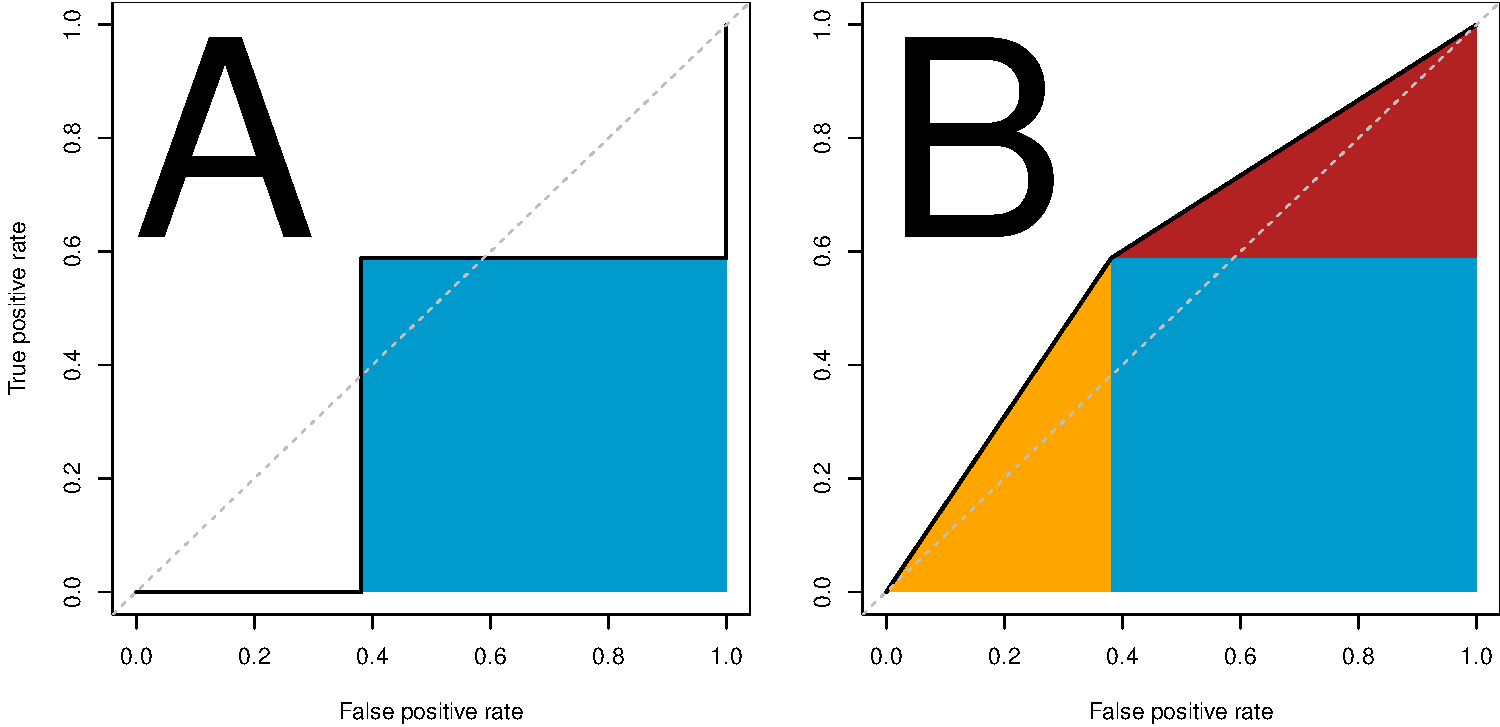
\includegraphics{main-1} 

}

\caption[ROC curve of the data in the simple concrete example]{ROC curve of the data in the simple concrete example.  Here we present a standard ROC curve, with the false positive rate or $1 - \text{specificity}$ on the x-axis and true positive rate or sensitivity on the y-axis.  The dotted line represents the identity. The shaded area in panel represents the AUC for the strict definition.  The additional shaded areas on panel B represent the AUC when accounting for ties.  }\label{fig:main}
\end{figure}
\end{CodeChunk}

\hypertarget{auc-calculation-in-statistical-software}{%
\subsection{AUC Calculation in Statistical
Software}\label{auc-calculation-in-statistical-software}}

To determine how these calculations are done in practice, we will
explore the estimated ROC curve and AUC from the implementations in the
following \texttt{R} \citep{rcore} packages: \pkg{ROCR} \citep{ROCR},
\pkg{caTools} \citep{caTools}, \pkg{pROC} \citep{pROC}, and \pkg{fbroc}
\citep{fbroc}. We will also show these agree with the Python
implementation in \texttt{sklearn.metrics} from \pkg{scikit-learn}
\citep{scikitlearn}, the Stata functions \texttt{roctab} and
\texttt{rocreg} \citep{bamber1975area, delong}, and the SAS software
functions \texttt{proc\ logistic} with \texttt{roc} and
\texttt{roccontrast} . We note that the majority of these functions all
count half the probability of ties, but differences exist in the
calculation of confidence intervals of AUC and note some inconsistent
behavior.

\hypertarget{auc-calculation-current-implementations}{%
\section{AUC Calculation: Current
Implementations}\label{auc-calculation-current-implementations}}

This section will present code and results from commonly-used
implementations of AUC estimation from R, Python, Stata, and SAS
software. We will note agreement with the definitions of AUC above and
any discrepancies. This section is not to be exhaustive, but give
examples how to calculate AUC in these software and show that these
definitions are consistently used in AUC analysis, primarily
\(\widehat{\text{AUC}}_{\text{w/ties}}\).

\hypertarget{r}{%
\subsection{R}\label{r}}

Here we will show the AUC calculation from the common \texttt{R}
packages for ROC analysis. We will show that each report the value
calculated in \(\text{AUC}_{\text{w/ties}}\). The \pkg{caTools}
\citep{caTools} package calculates AUC using the \texttt{colAUC}
function, taking in predictions as \texttt{x} and the binary ground
truth labels as \texttt{y}:

\begin{CodeChunk}

\begin{CodeInput}
R> library(caTools)
R> colAUC(x, y)
\end{CodeInput}

\begin{CodeOutput}
             [,1]
0 vs. 1 0.6036415
\end{CodeOutput}
\end{CodeChunk}

which reports \(\text{AUC}_{\text{w/ties}}\).

In \pkg{ROCR} package \citep{ROCR}, one must create a \code{prediction}
object with the \code{prediction} function, which can calculate a series
of measures. AUC is calculated from a \code{performance} function,
giving a \code{performance} object, and giving the \texttt{"auc"}
measure. We can then extract the AUC as follows:

\begin{CodeChunk}

\begin{CodeInput}
R> library(ROCR)
R> pred = prediction(x, y)
R> auc.est = performance(pred, "auc")
R> auc.est@y.values[[1]]
\end{CodeInput}

\begin{CodeOutput}
[1] 0.6036415
\end{CodeOutput}
\end{CodeChunk}

which reports \(\text{AUC}_{\text{w/ties}}\). We see this agrees with
the plot from \texttt{ROCR} in Figure \ref{ROCR}.

The \pkg{pROC} \citep{pROC} package calculates AUC using the
\texttt{roc} function:

\begin{CodeChunk}

\begin{CodeInput}
R> library(pROC)
R> pROC.roc = pROC::roc(predictor = x, response = y)
R> pROC.roc[["auc"]]
\end{CodeInput}

\begin{CodeOutput}
Area under the curve: 0.6036
\end{CodeOutput}
\end{CodeChunk}

which reports \(\text{AUC}_{\text{w/ties}}\) and agrees with the plot
from \texttt{pROC} in Figure \ref{pROC}.

The \pkg{fbroc} package calculates the ROC using the
\texttt{fbroc::boot.roc} and \texttt{fbroc::perf} functions. The package
has 2 strategies for dealing with ties, which we will create 2 different
objects \texttt{fbroc.default}, using the default strategy (strategy 2),
and alternative strategy (strategy 1, \texttt{fbroc.alternative}):

\begin{CodeChunk}

\begin{CodeInput}
R> library(fbroc)
R> fbroc.default = boot.roc(x, as.logical(y), 
R+                          n.boot = 1000, tie.strategy = 2)
R> auc.def = perf(fbroc.default, "auc")
R> auc.def[["Observed.Performance"]]
\end{CodeInput}

\begin{CodeOutput}
[1] 0.6036415
\end{CodeOutput}

\begin{CodeInput}
R> fbroc.alternative = boot.roc(x, as.logical(y), 
R+                              n.boot = 1000, tie.strategy = 1)
R> auc.alt = perf(fbroc.alternative, "auc")
R> auc.alt[["Observed.Performance"]]
\end{CodeInput}

\begin{CodeOutput}
[1] 0.6036415
\end{CodeOutput}
\end{CodeChunk}

which both report \(\text{AUC}_{\text{definition}}\), identical results
to above and agrees with the plot from \texttt{fbroc} in Figure
\ref{fbroc2}, which is for strategy 2.

Although the output is the same, these strategies for ties are different
for the plotting for the ROC curve, which we see in Figure
\ref{fig:fbrocs}. The standard error calculation for both strategies use
the second strategy (Fawcett's ``pessimistic'' approach), which is
described in a blog post
(\url{https://www.epeter-stats.de/roc-curves-and-ties/}) and can be seen
in the shaded areas of the panels. Thus, we see that using either tie
strategy results in the same estimate of AUC
(\(\text{AUC}_{\text{w/ties}}\)), but using tie strategy 1 results in a
plot which would reflect an AUC of \(\text{AUC}_{\text{definition}}\)
(Figure \ref{fig:fbroc1}), which seem to disagree. This result is
particularly concerning because the plot should agree with the
interpretation of AUC.

\hypertarget{python}{%
\subsection{Python}\label{python}}

In Python, we will use the implementation in \texttt{sklearn.metrics}
from \pkg{scikit-learn} \citep{scikitlearn}. We will use the \texttt{R}
package \texttt{reticulate} \citep{reticulate}, which will provide an
Python interface to \texttt{R}. Here we use the \texttt{roc\_curve} and
\texttt{auc} functions from \pkg{scikit-learn} and output the estimated
AUC:

\begin{CodeChunk}

\begin{CodeInput}
R> # Adapted from https://qiita.com/bmj0114/items/460424c110a8ce22d945
R> library(reticulate)
R> sk = import("sklearn.metrics")
R> py.roc.curve = sk$roc_curve(y_score = x, y_true = y)
R> names(py.roc.curve) = c("fpr", "tpr", "thresholds")
R> py.roc.auc = sk$auc(py.roc.curve$fpr, py.roc.curve$tpr)
R> py.roc.auc
\end{CodeInput}

\begin{CodeOutput}
[1] 0.6036415
\end{CodeOutput}
\end{CodeChunk}

which reports \(\text{AUC}_{\text{w/ties}}\). Although we have not
exhaustively shown Python reports \(\text{AUC}_{\text{w/ties}}\),
\texttt{scikit-learn} is one of the most popular Python modules for
machine learning and analysis. We can use \texttt{matplotlib}
\citep{matplotlib} to plot FPR and TPR from the \texttt{py.roc.curve}
object, which we see in Figure \ref{fig:python}, which uses a linear
interpolation by default and agrees with \(\text{AUC}_{\text{w/ties}}\).

\hypertarget{sas-software}{%
\subsection{SAS Software}\label{sas-software}}

In SAS software (version 9.4 for Unix) \citep{sas}, let us assume we
have a data set named \texttt{roc} loaded with the variables/columns of
\texttt{x} and \texttt{y} as above. The following commands will produce
the ROC curve in Figure \ref{sas}:

\begin{CodeChunk}

\begin{CodeInput}
R>   proc logistic data=roc;
R+       model y(event='1') = x;
R+       roc; roccontrast;
R+       run;      
\end{CodeInput}
\end{CodeChunk}

The resulting output reports \(\text{AUC}_{\text{w/ties}}\), along with
a confidence interval. The calculations can be seen in the SAS User
Guide
(\url{https://support.sas.com/documentation/cdl/en/statug/63033/HTML/default/viewer.htm\#statug_logistic_sect040.htm}),
which includes the addition of the probability of ties.

\hypertarget{stata}{%
\subsection{Stata}\label{stata}}

In Stata (StatCorp, College Station, TX, version 13) \citep{stata}, let
us assume we have a data set with the variables/columns of \texttt{x}
and \texttt{y} as above.

The function \texttt{roctab} is one common way to calculate an AUC:

\begin{CodeChunk}

\begin{CodeInput}
R> roctab x y
\end{CodeInput}
\end{CodeChunk}

which agrees with the calculation based on
\(\text{AUC}_{\text{w/ties}}\) and agrees with the estimates from above.
One can also calculate the AUC using the \texttt{rocreg} function:

\begin{CodeChunk}

\begin{CodeInput}
R> rocreg y x, nodots auc
\end{CodeInput}
\end{CodeChunk}

which agrees with the definition of \(\text{AUC}_{\text{definition}}\)
and is different from the output from \texttt{roctab}. The variance of
the estimate is based on a bootstrap estimate, but the point estimate
will remain the same regardless of using the bootstrap or not. This
disagreement of estimates is concerning as the reported estimated AUC
may be different depending on the command used in the estimation.

Using \texttt{rocregplot} after running this estimation, we see can
create an ROC curve, which is shown in Figure \ref{fig:stata}. We see
that the estimated ROC curve coincides with the estimated AUC from
\texttt{rocreg} (\(\text{AUC}_{\text{definition}}\)) and the blue
rectangle in Figure \ref{fig:main}. Thus, \texttt{roctab} is one of the
most common ways in Stata to estimate AUC, but does not agree with the
common way to plot ROC curves.

\begin{figure}
     \centering
     \subfloat[][Stata ROC Plot ]{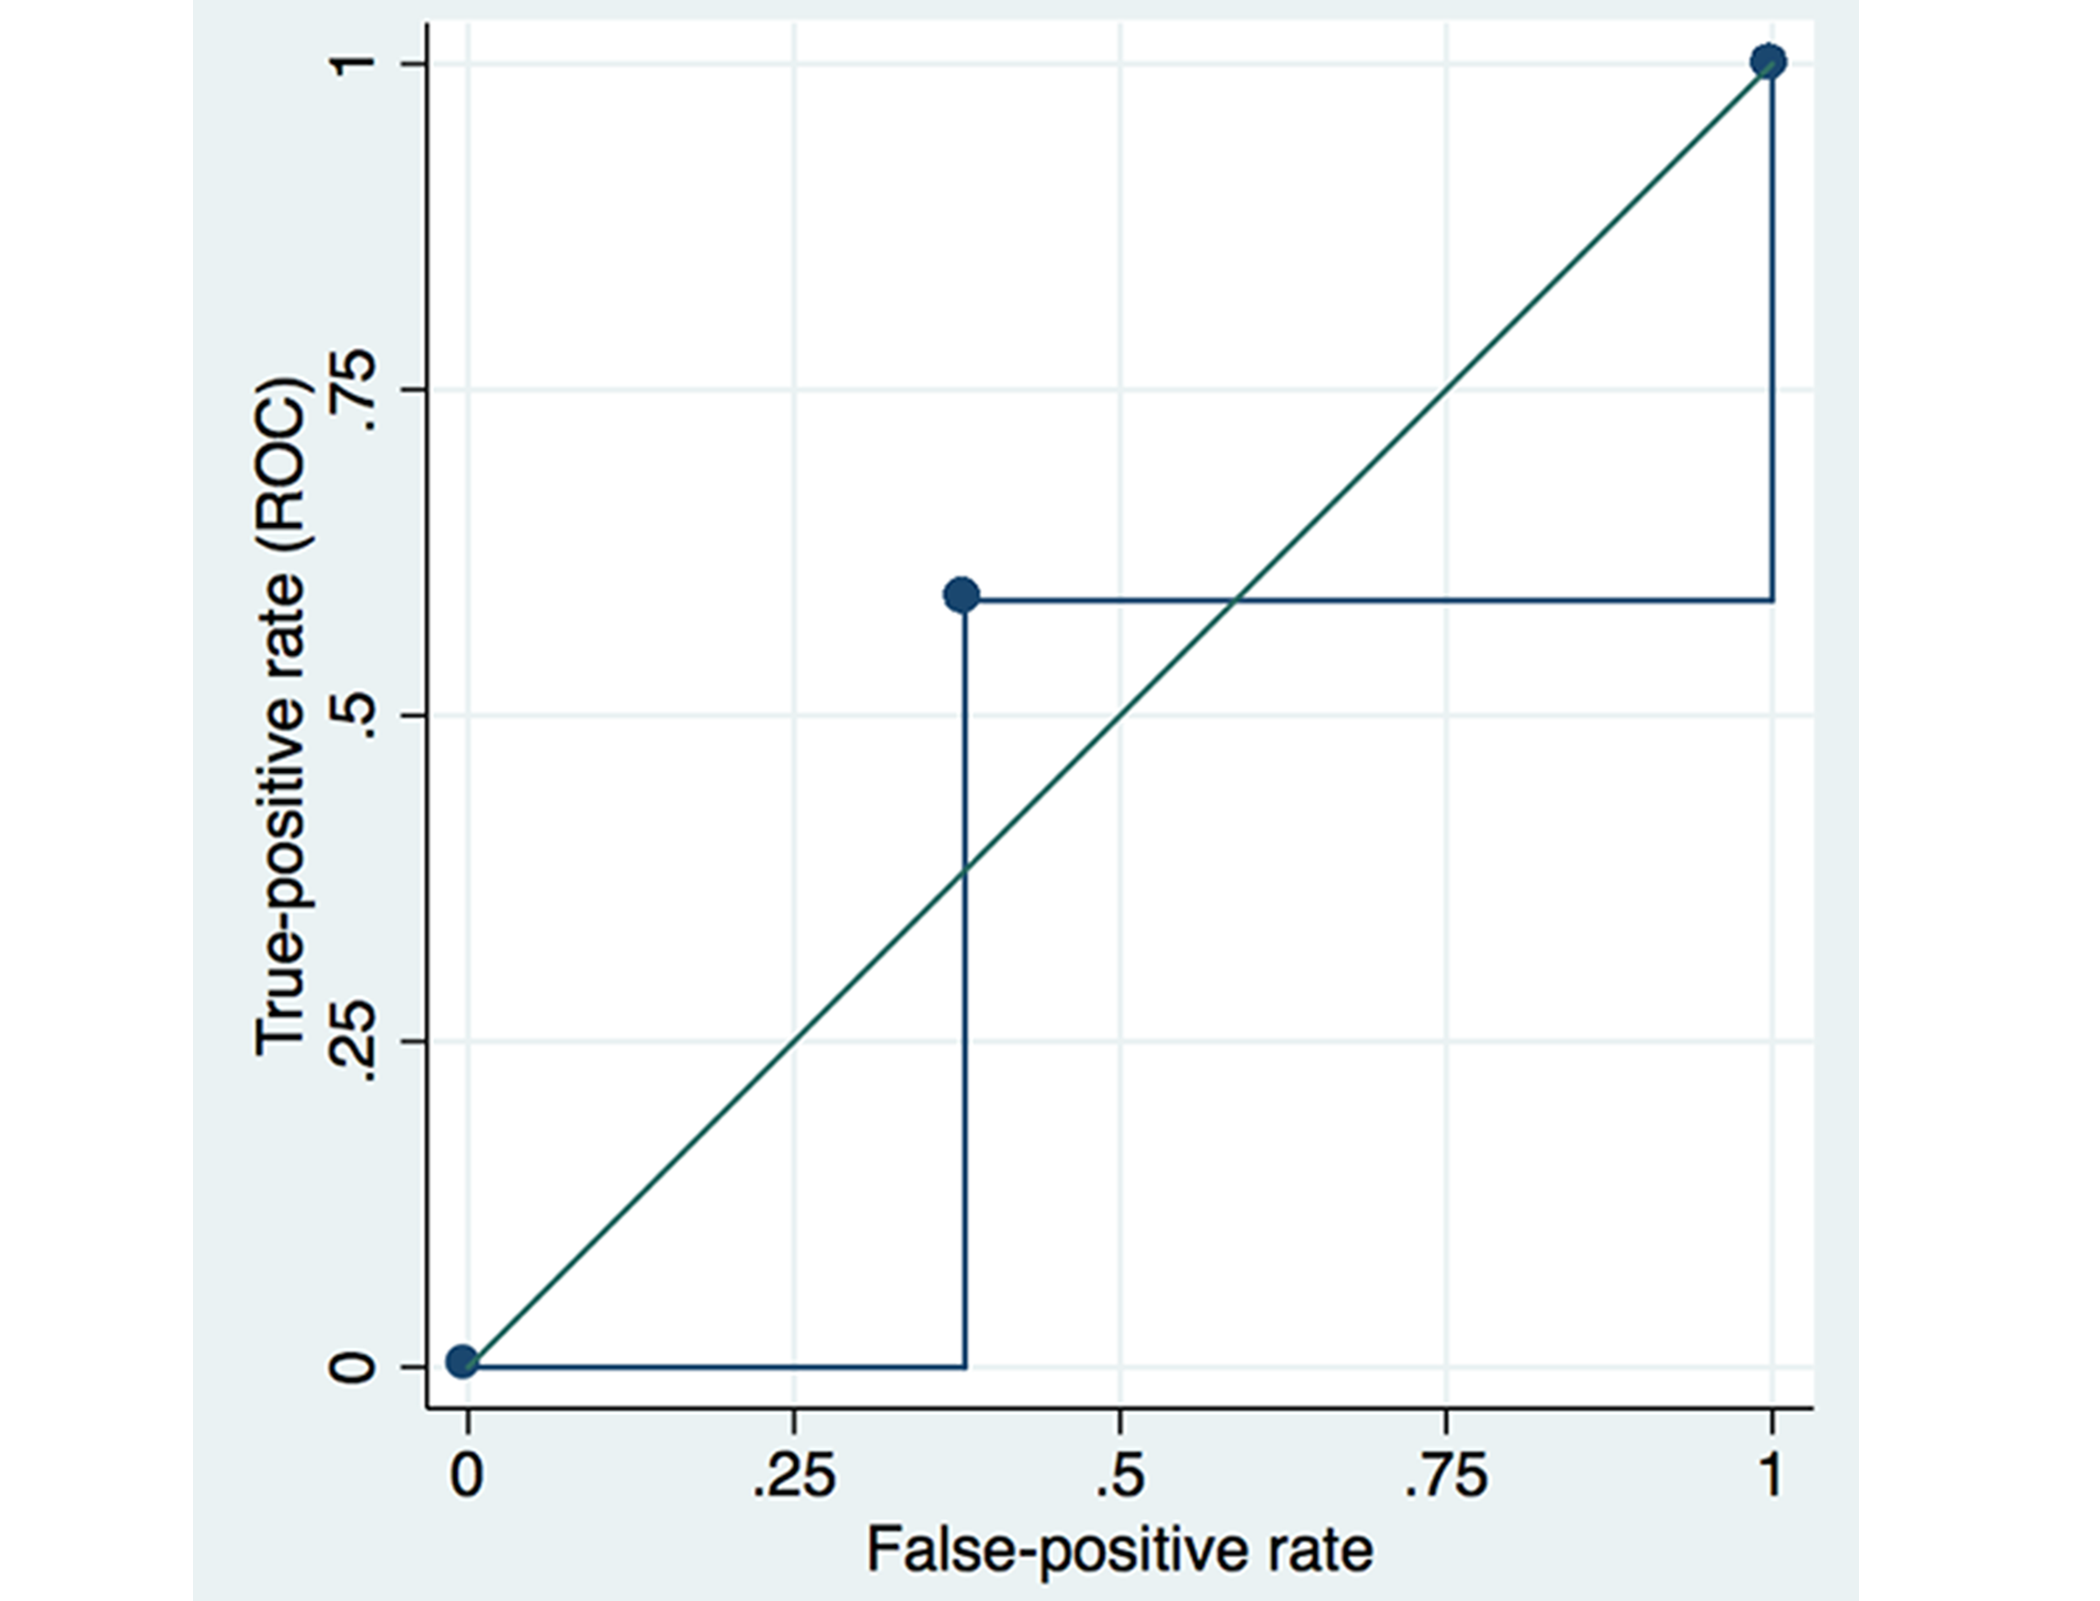
\includegraphics[width=0.32\linewidth]{stata_roc_cropped.png}\label{fig:stata}}
     \subfloat[][Python ROC Plot from scikit-learn]{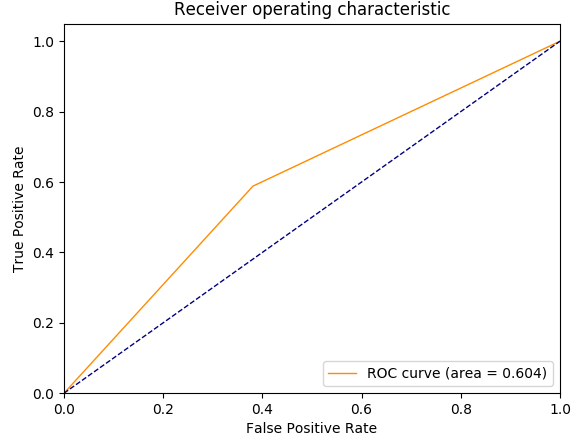
\includegraphics[width=0.32\linewidth]{python_roc_cropped.png}\label{fig:python}} 
     \subfloat[][SAS ROC Plot ]{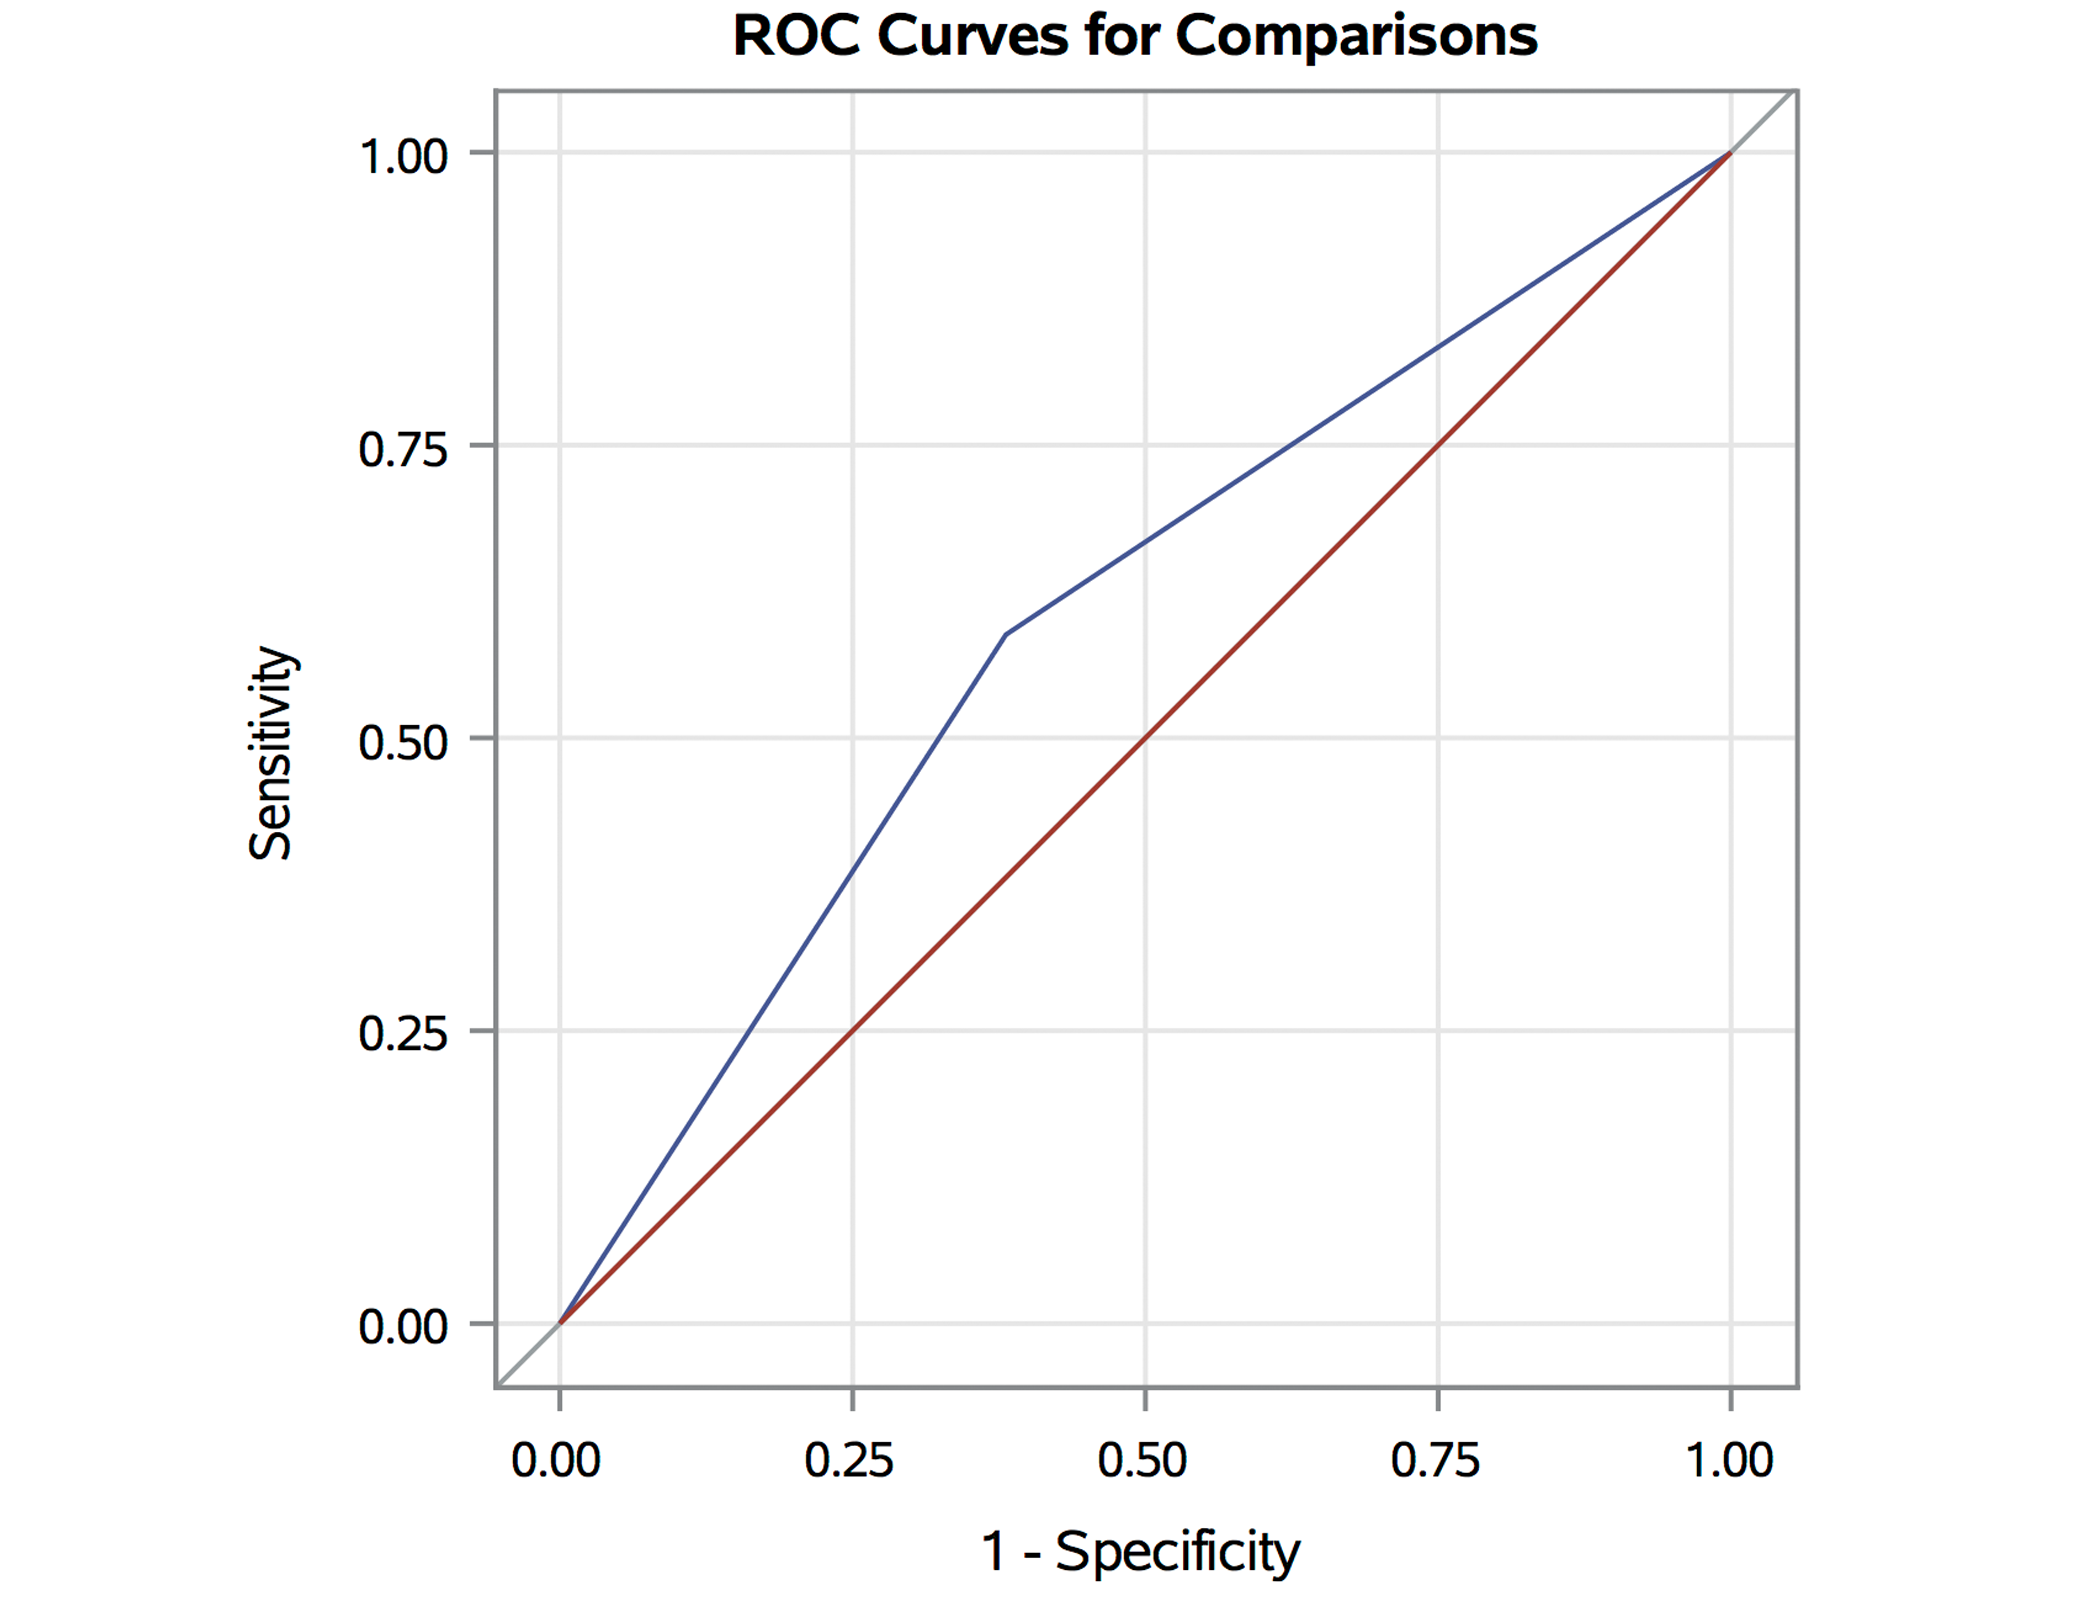
\includegraphics[width=0.32\linewidth]{sas_cropped.png}\label{sas}} \\
     \subfloat[][ROCR ROC plot ]{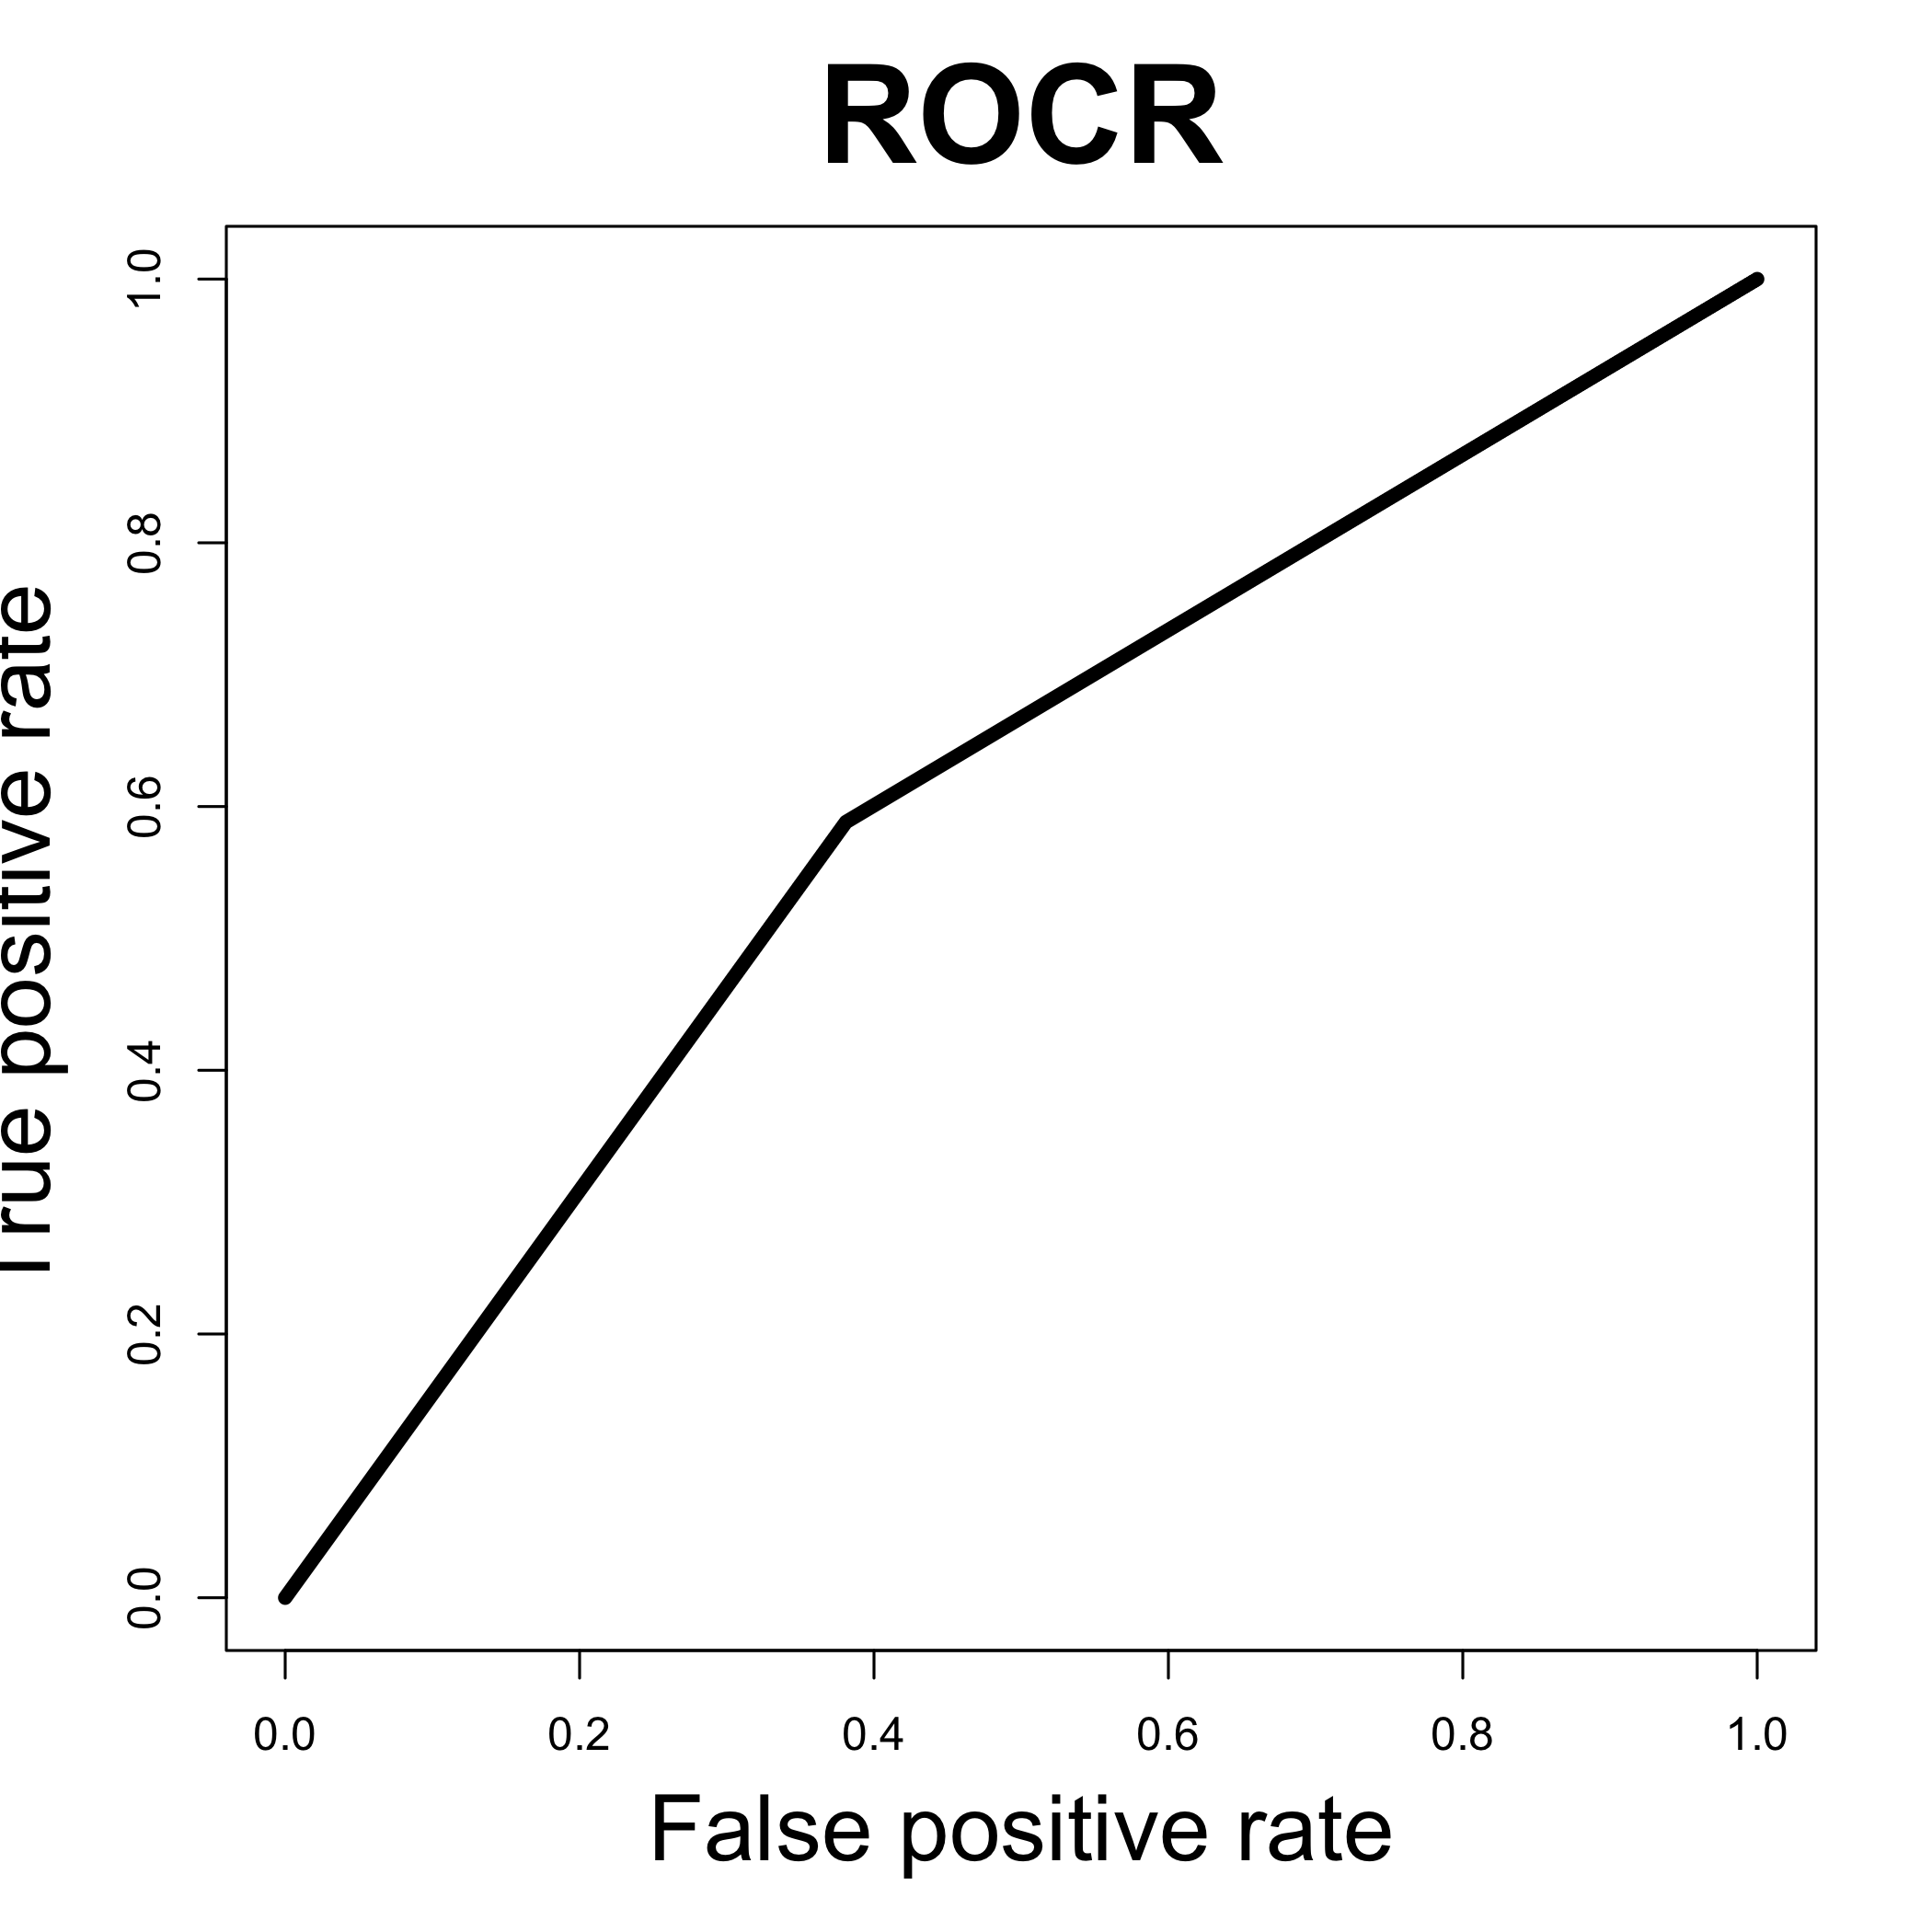
\includegraphics[width=0.32\linewidth]{ROCR.png}\label{ROCR}}
     \subfloat[][pROC ROC plot ]{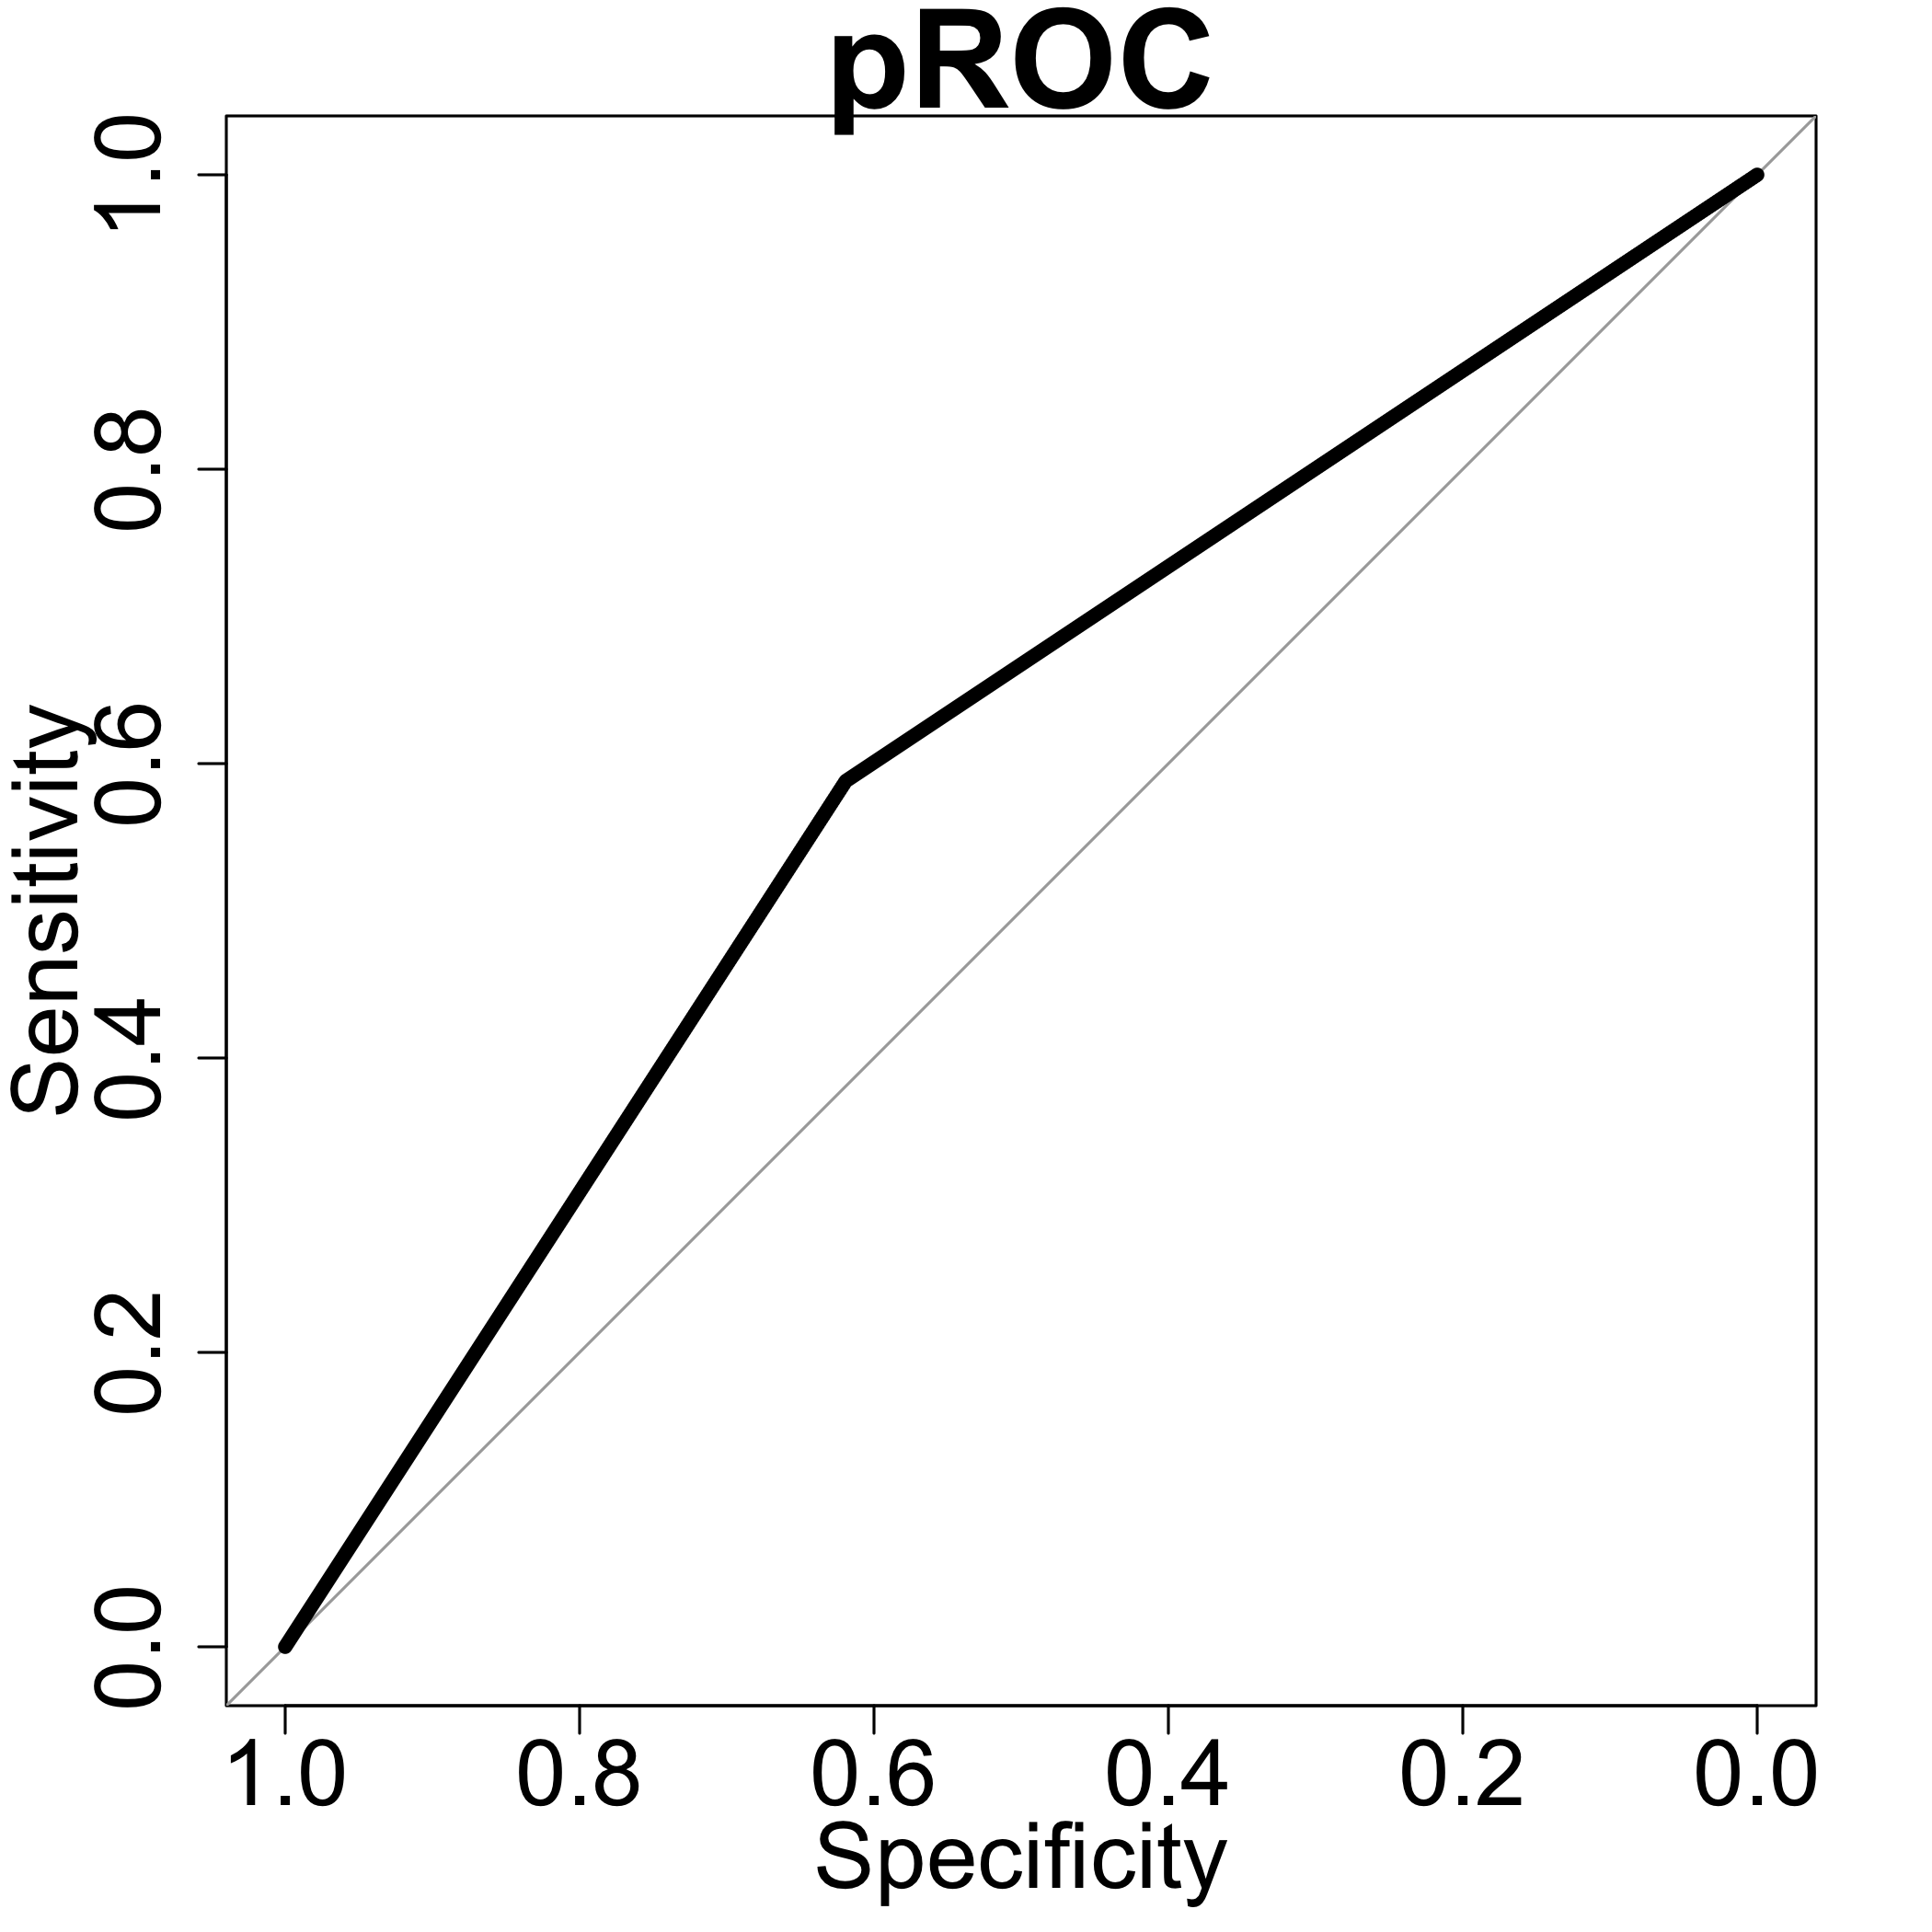
\includegraphics[width=0.32\linewidth]{pROC.png}\label{pROC}}
     \subfloat[][fbroc Strategy 2 (default)
]{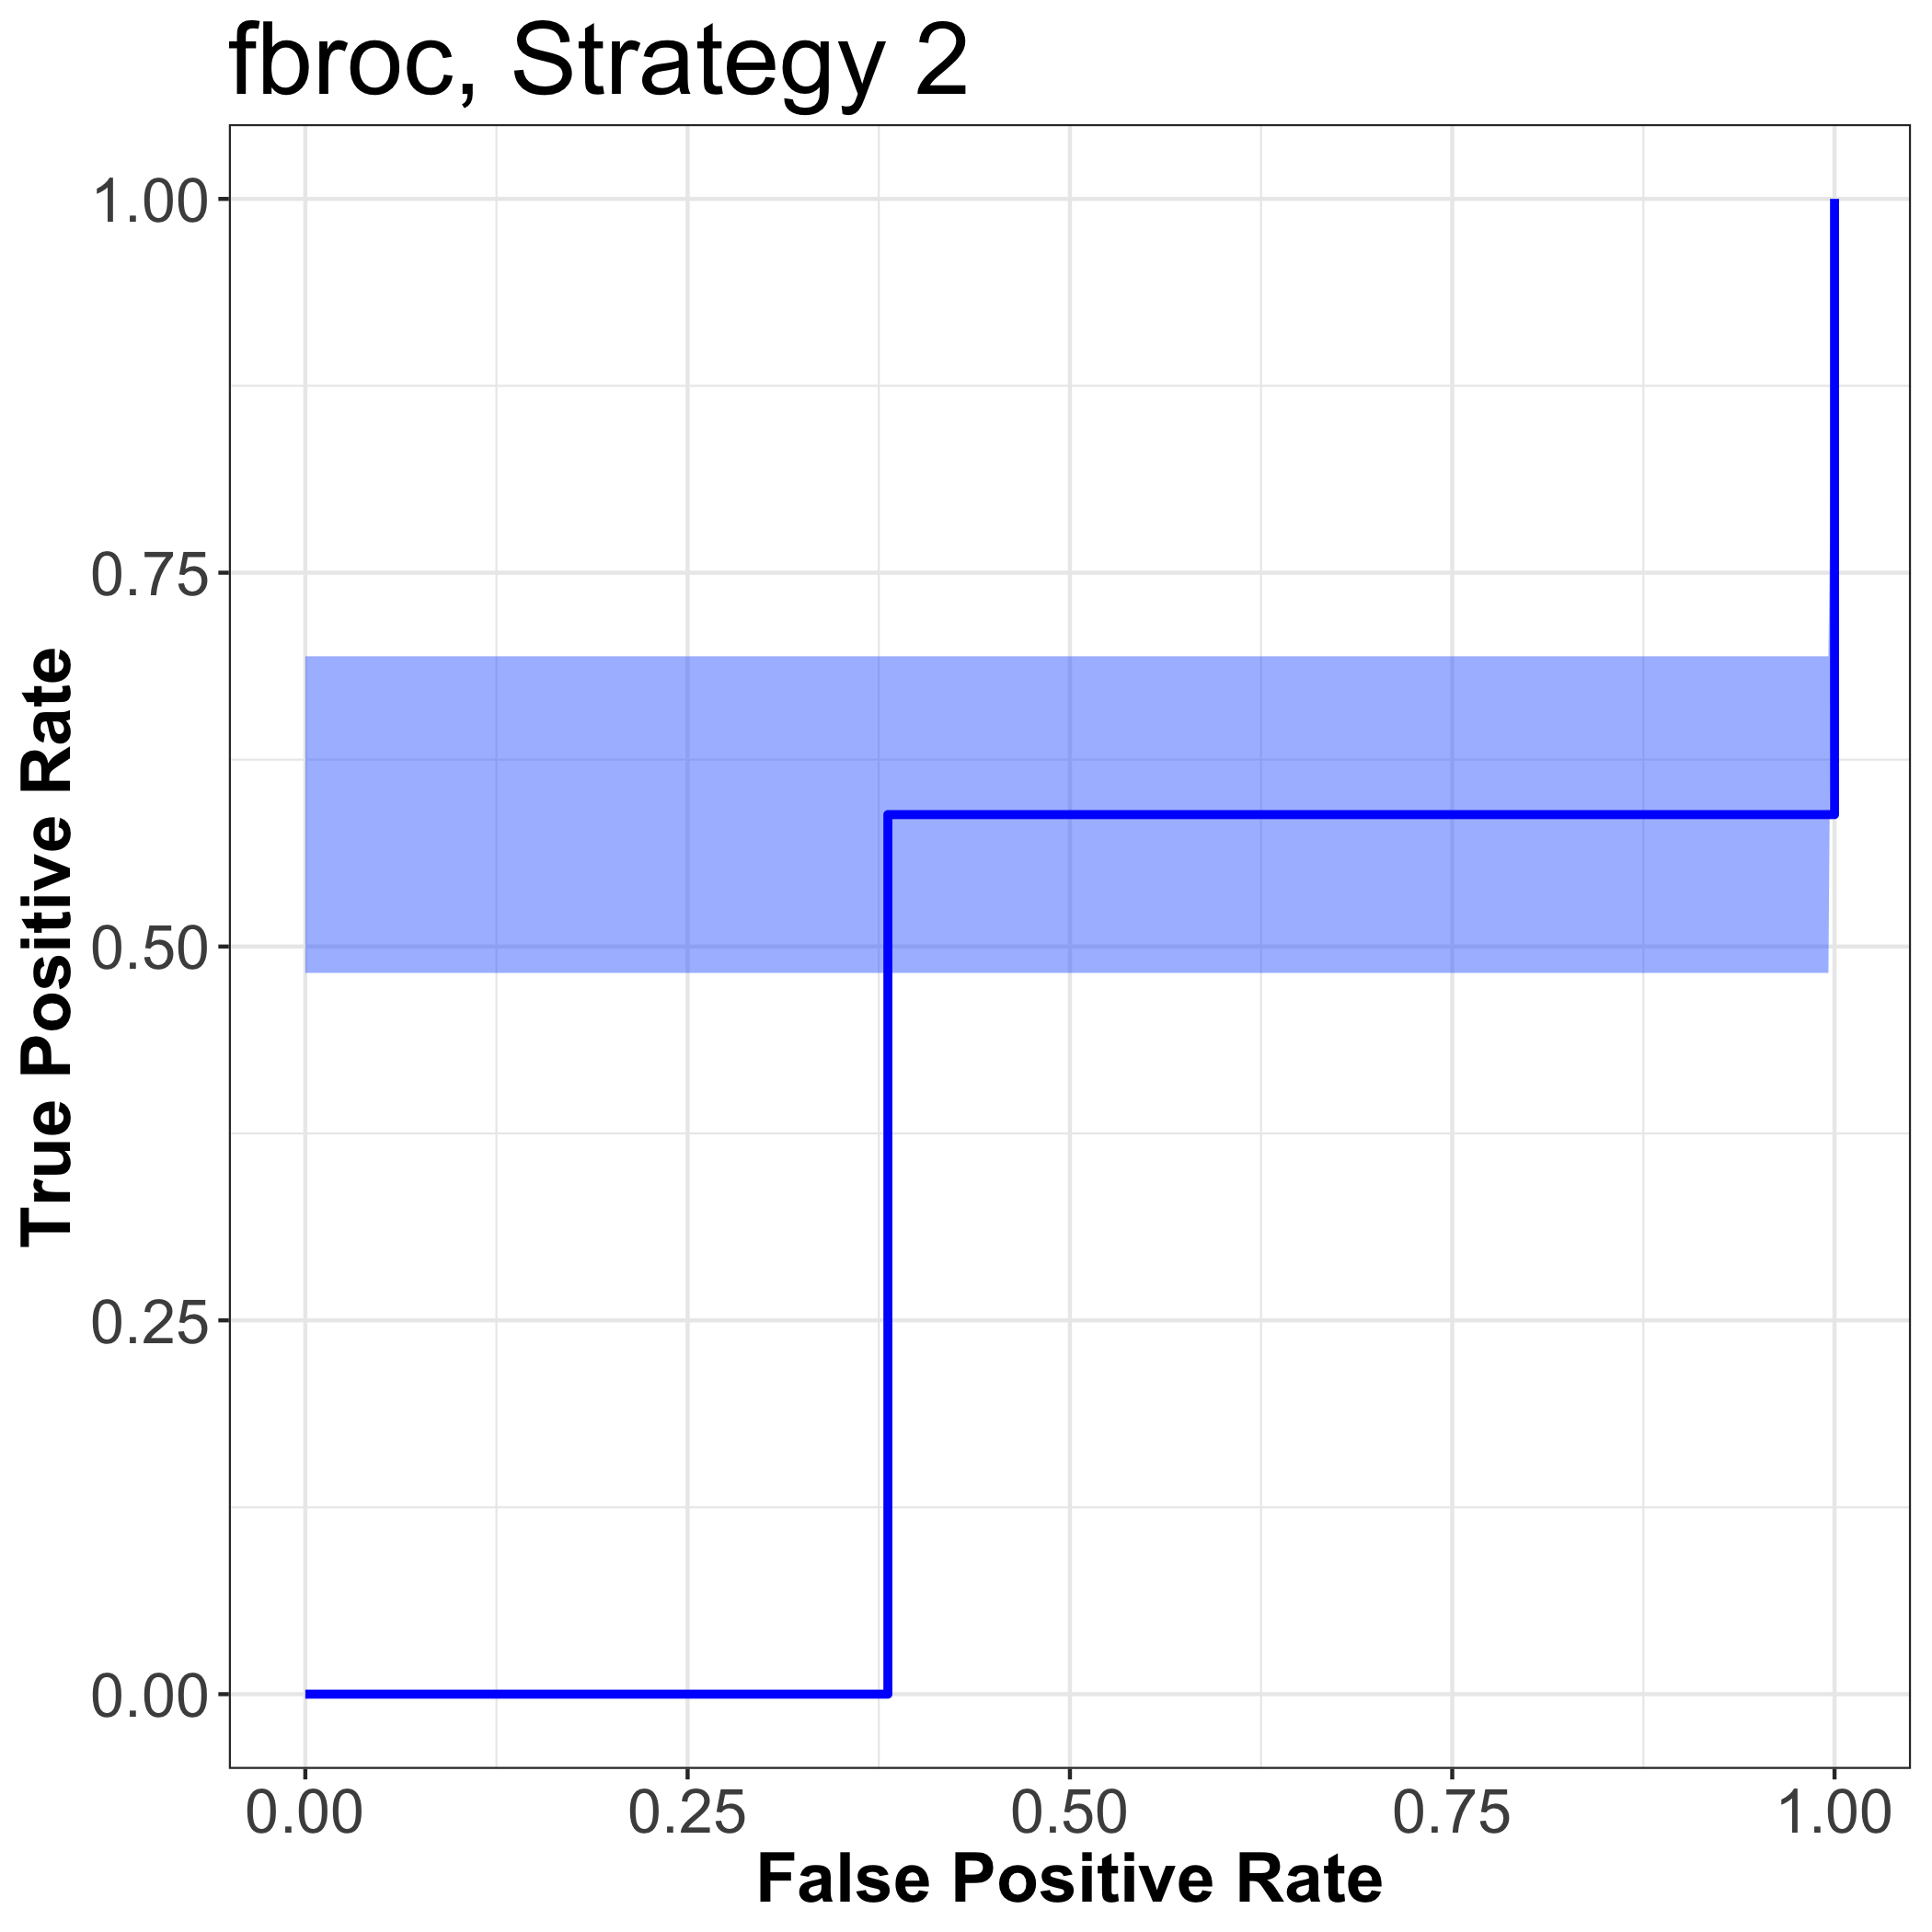
\includegraphics[width=0.32\linewidth]{fbroc2.png}\label{fbroc2}}
     \caption{Comparison of different ROC curves for different  \code{R} packages,  \code{scikit-learn} from  \code{Python},  \code{SAS}, and  \code{Stata}.  Each line represents the ROC curve, which corresponds to an according area under the curve (AUC).  The blue shading represents the confidence interval for the ROC curve in the  \code{fbroc} package.  Also, each software represents the curve as the false positive rate versus the true positive rate, though the  \code{pROC} package calls it sensitivity and specificity (with flipped axes).  Some put the identity line where others do not.  Overall the difference of note as to whether the ROC curve is represented by a step or a linear function. Using the first tie strategy for ties (non-default) in  \code{fbroc} gives the same confidence interval but an ROC curve using linear interpolation.}
     \label{fig:rocs}
\end{figure}

Thus, we see in Figure \ref{fig:rocs} that all ROC curves are
interpolated with a linear interpolation, which coincides with the
calculation based on \(\text{AUC}_{\text{w/ties}}\), except for the
Stata ROC curve, which interpolates using a step function and coincides
with \(\text{AUC}_{\text{definition}}\). The confidence interval
estimate of the ROC curve for \texttt{fbroc}, which is shaded in blue in
Figure \ref{fbroc2}, corresponds to variability based on
\(\text{AUC}_{\text{definition}}\), though it shows the ROC curve based
on \(\text{AUC}_{\text{w/ties}}\).

\begin{figure}
     \centering
     \subfloat[][fbroc Strategy 1  ]{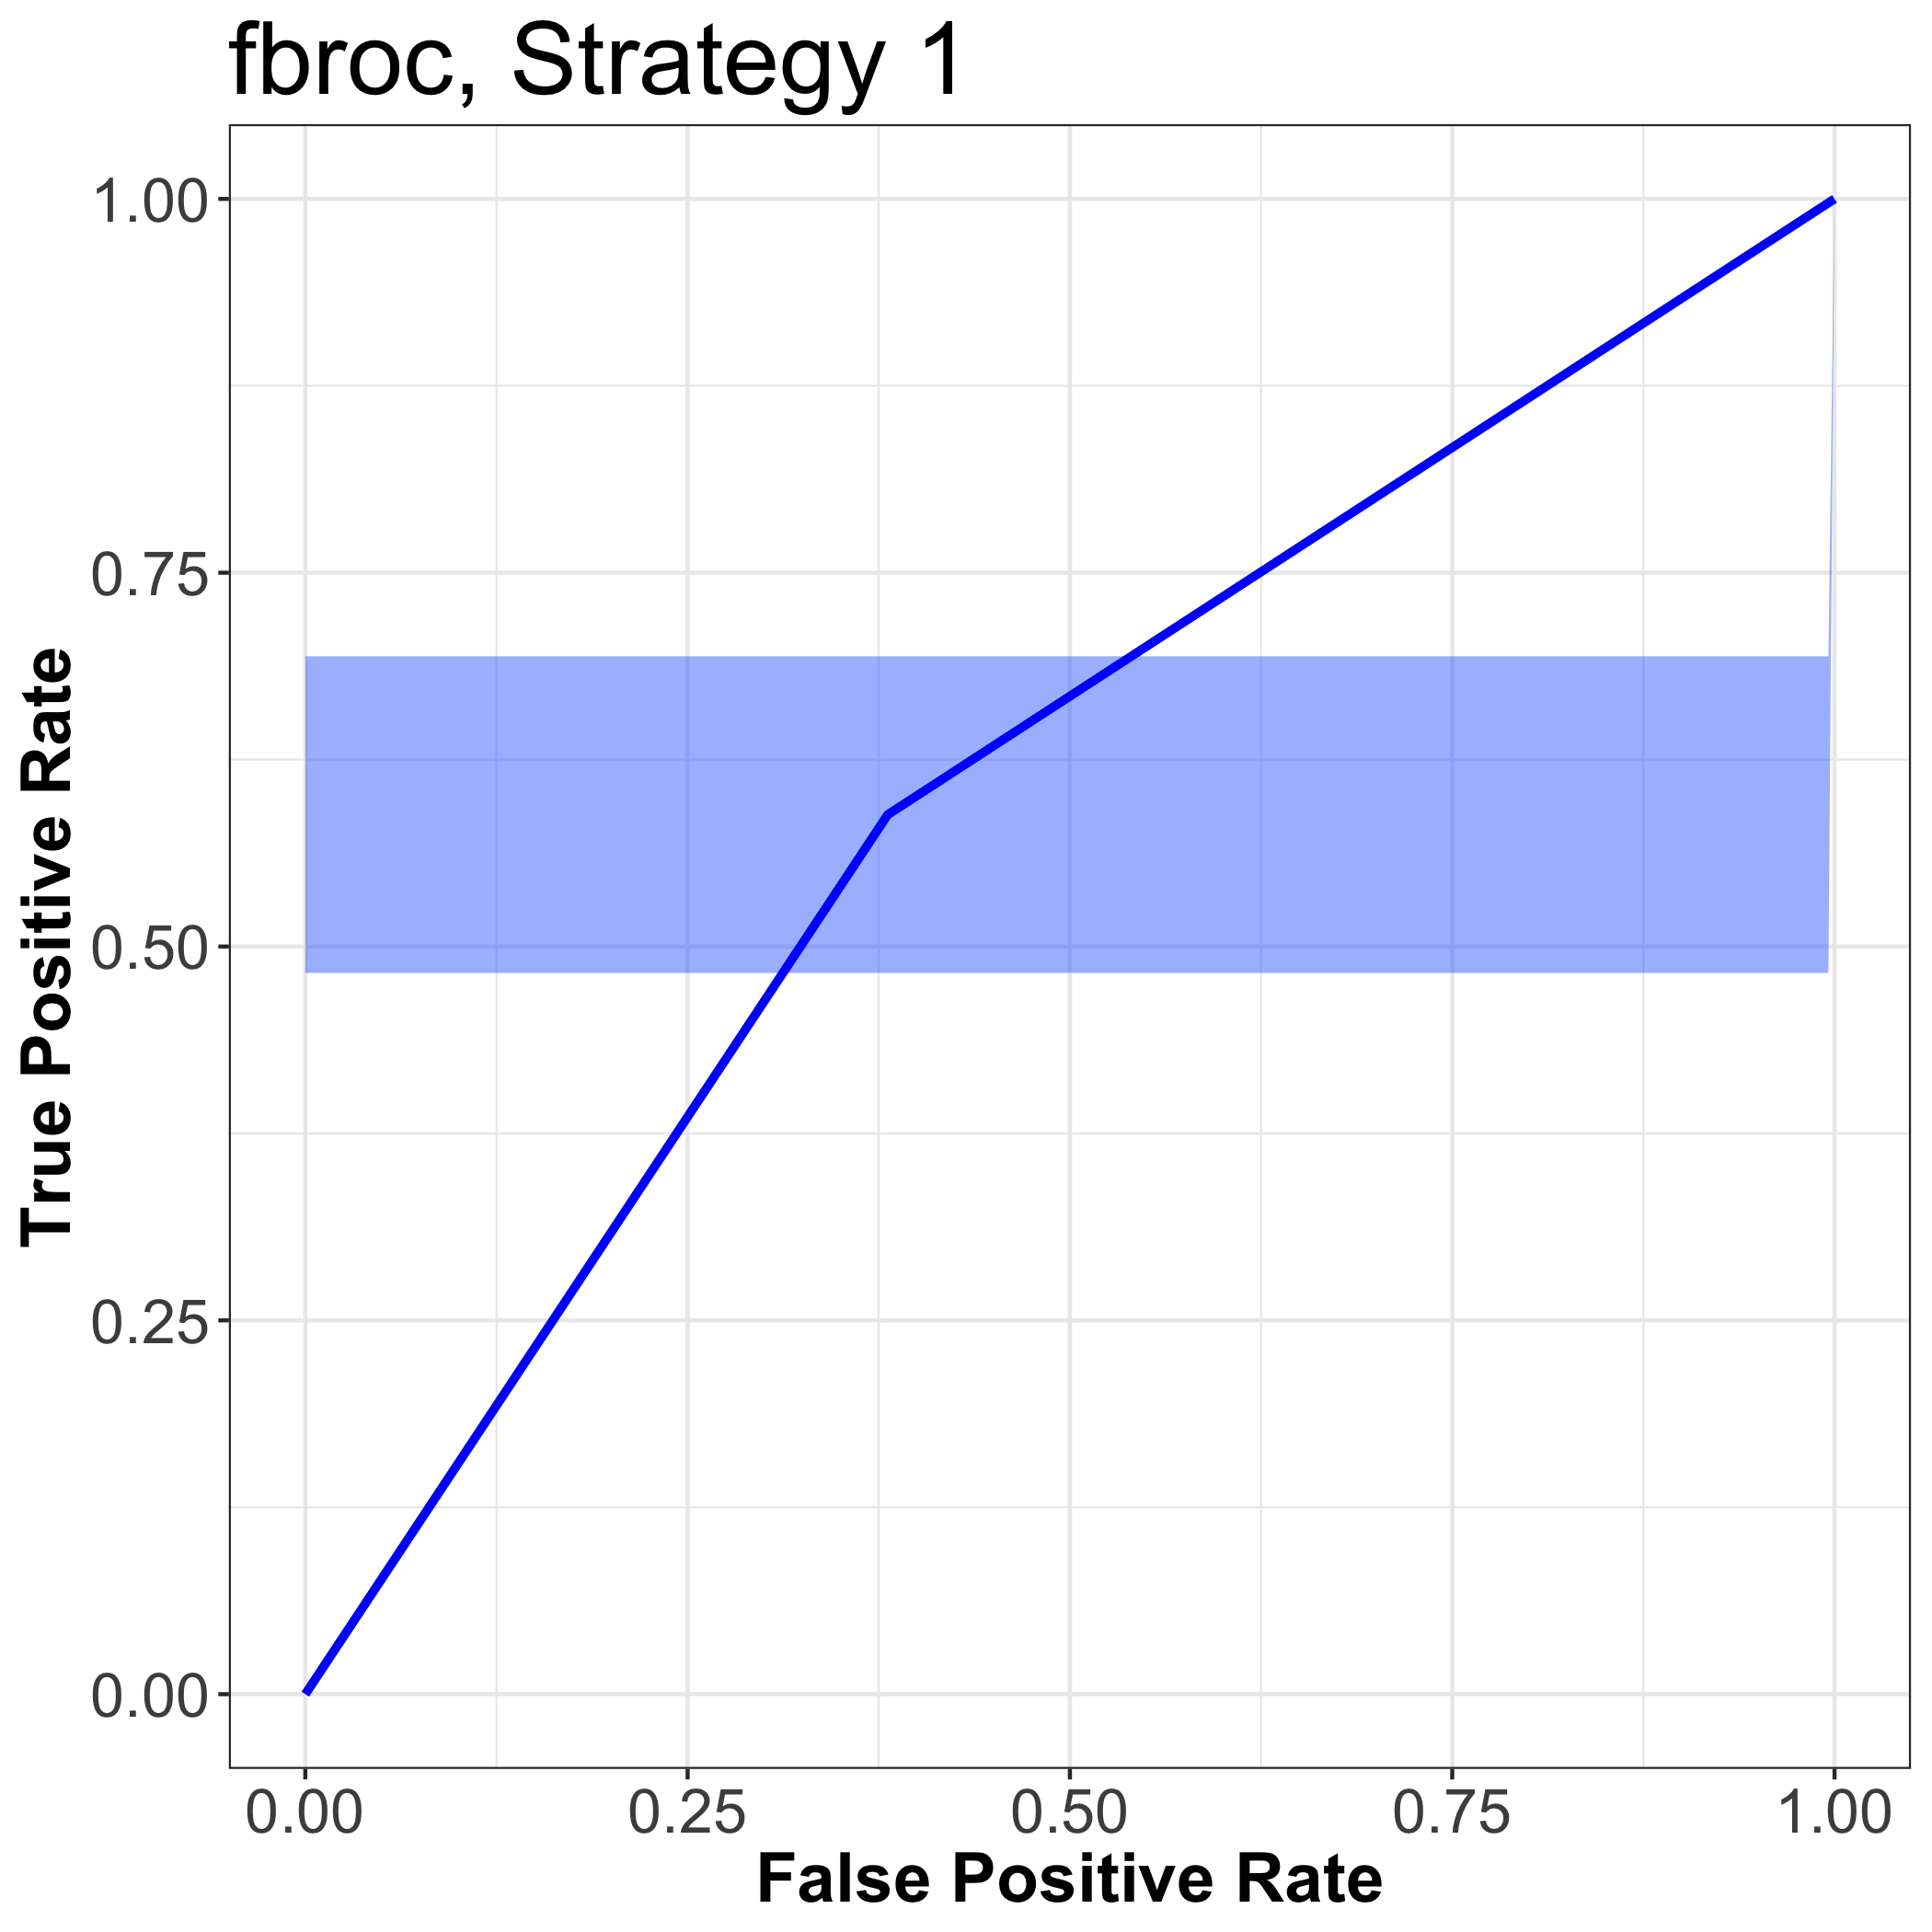
\includegraphics[width=0.48\linewidth]{fbroc1.png}\label{fig:fbroc1}}
     \subfloat[][fbroc Strategy 2 (default)
]{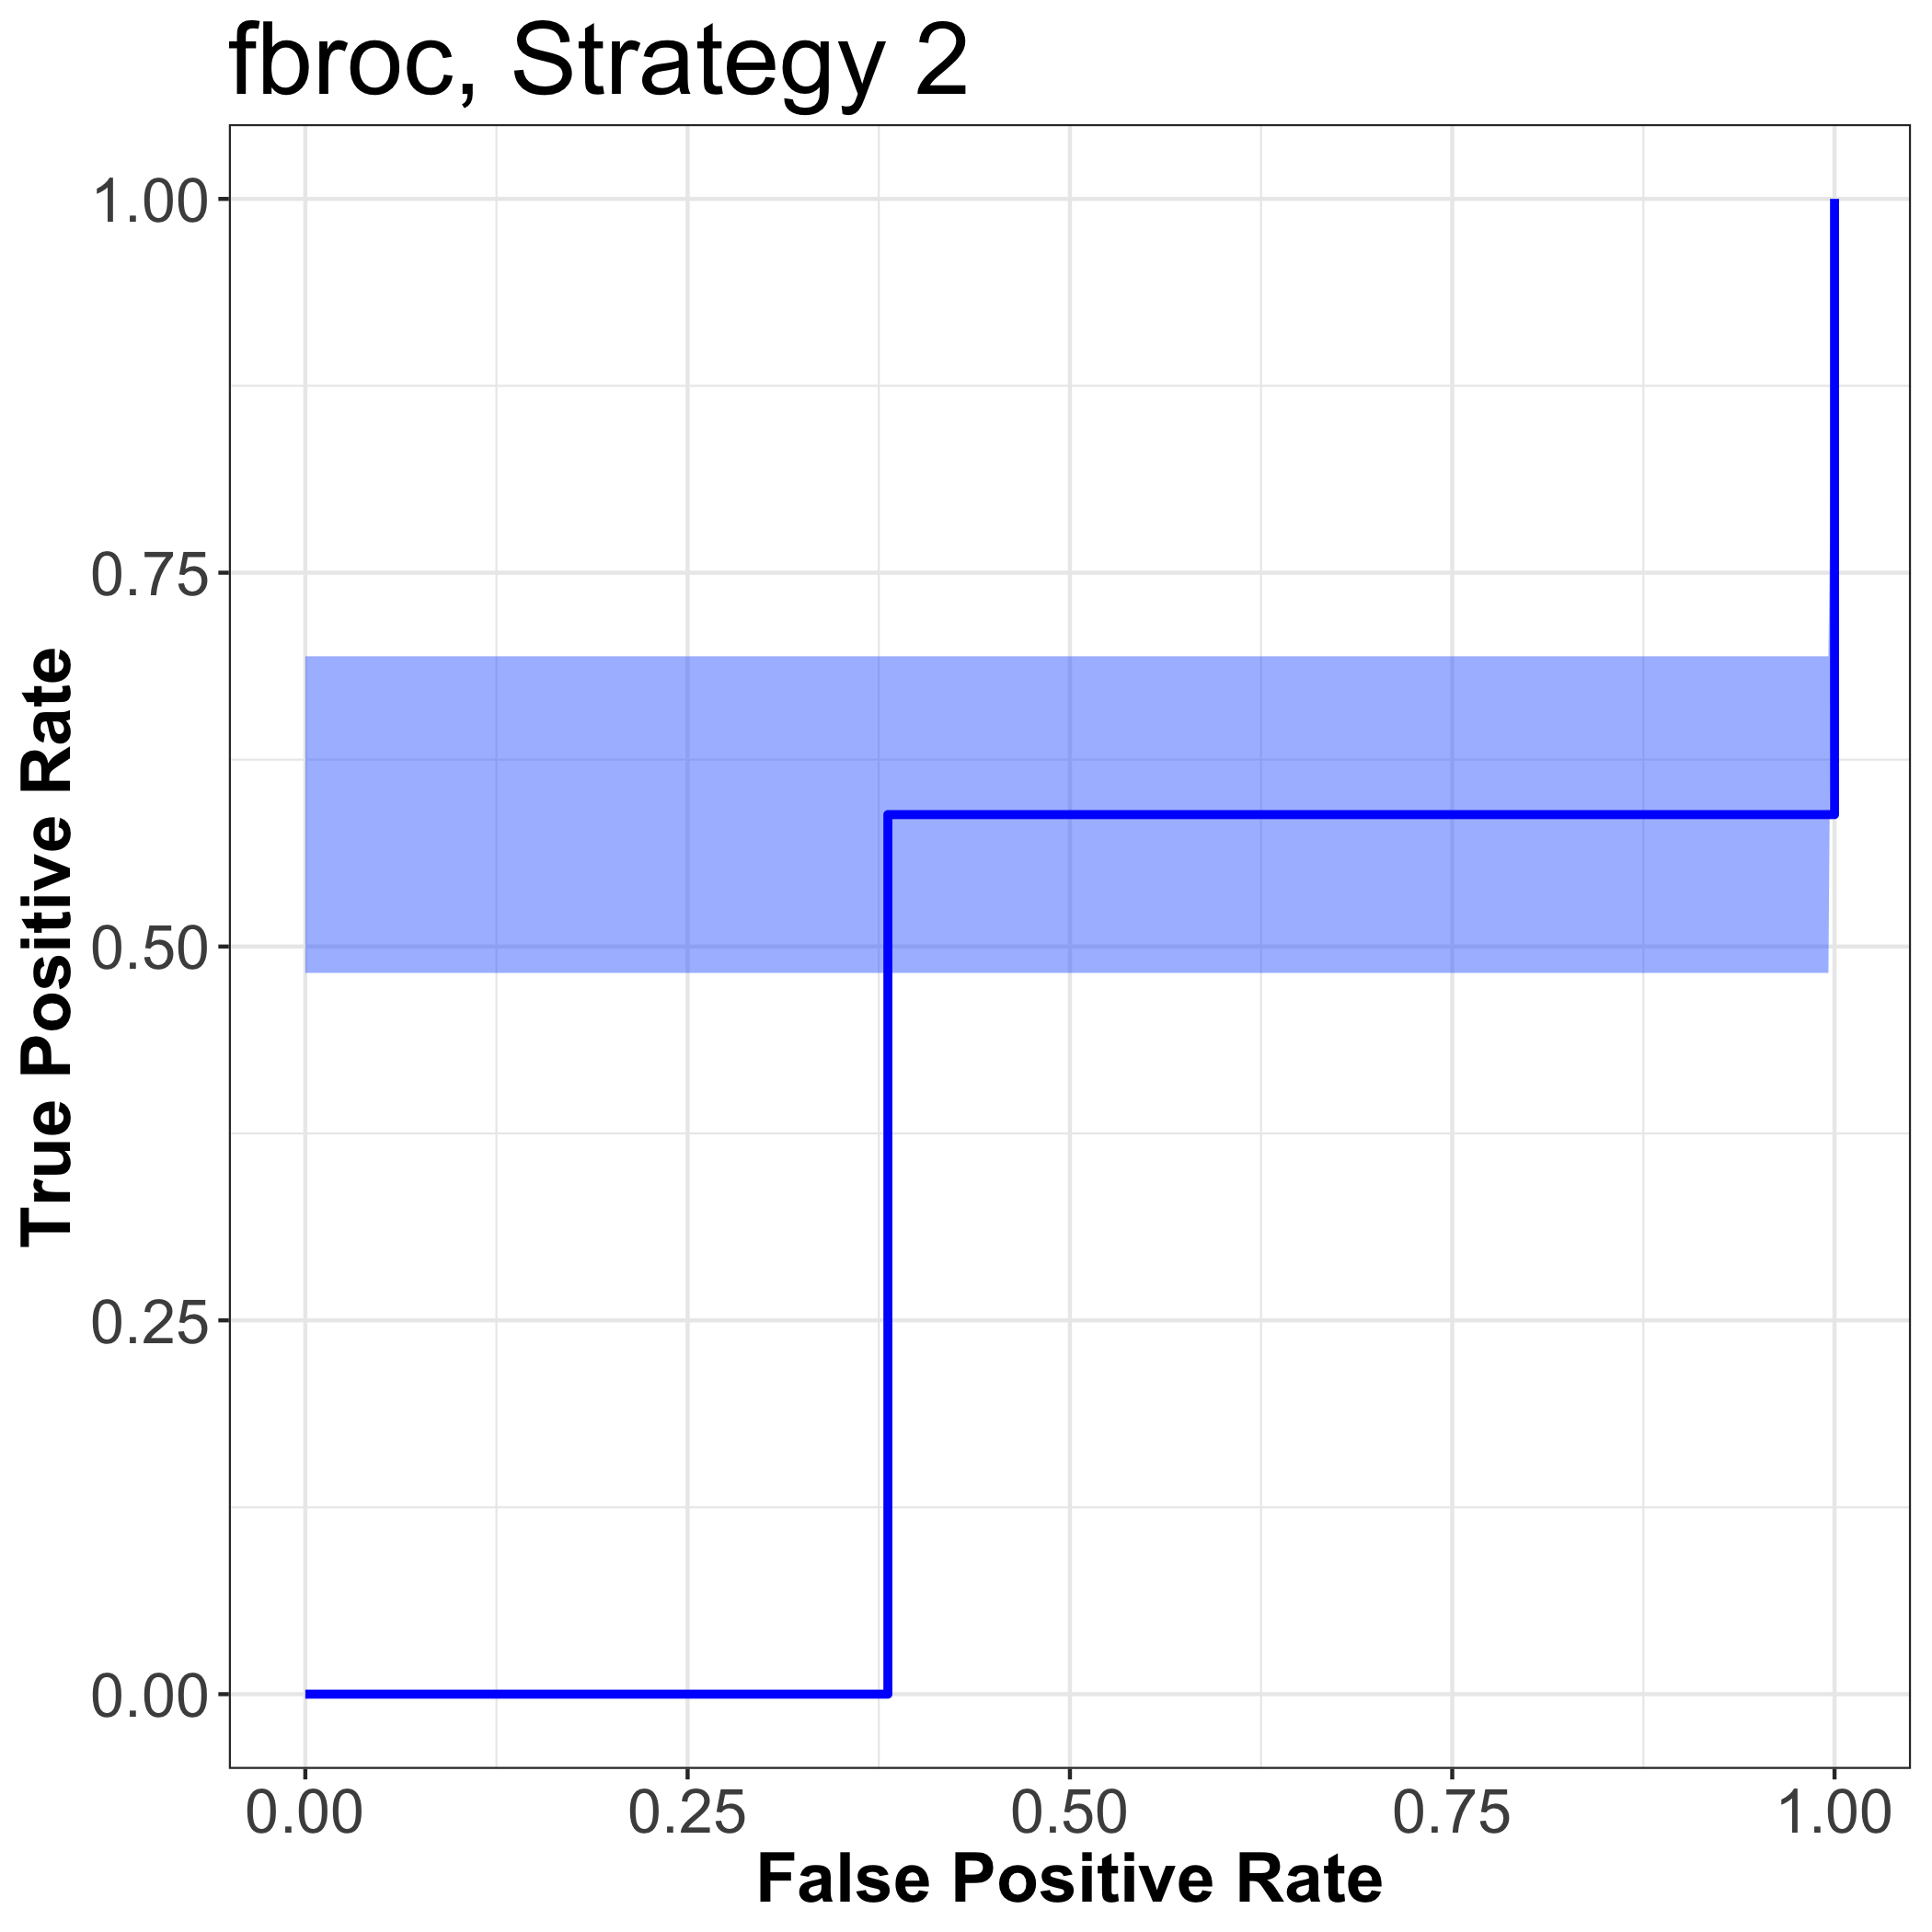
\includegraphics[width=0.48\linewidth]{fbroc2.png}\label{fig:fbroc2}}
     \caption{Comparison of different strategies for ties in the  \code{fbroc} package.  The blue shading represents the confidence interval for the ROC curve.  Overall the difference of note as to whether the ROC curve is represented by a step or a linear function. Using the first tie strategy for ties (non-default) in \code{fbroc} gives the same confidence interval as the second strategy but an ROC curve using linear interpolation, which may give an inconsistent combination of estimate and confidence interval.}
     \label{fig:fbrocs}
\end{figure}

Figure \ref{fig:fbrocs} shows that using the different tie strategies
gives a linear (strategy 2, default, panel \subref{fig:fbroc2},
duplicated) or step function/constant (strategy 1, panel
\subref{fig:fbroc1}) interpolation. In each tie strategy, however, the
AUC is estimated to be the same. Therefore, tie strategy 1 may give an
inconsistent combination of AUC estimate and ROC representation.

\hypertarget{conclusion}{%
\section{Conclusion}\label{conclusion}}

We have shown how the ROC curve is plotted and AUC is estimated in
common statistical software when using a unviariate binary predictor.
There are inconsistencies across software platforms, such as \texttt{R}
and Stata, and even within some packages, such as \texttt{fbroc}. We
believe these calculations do not reflect the discreteness of the data.
We agree that using a binary predictor in an ROC analysis may not be
appropriate, but we note that researchers and users will perform this.
Therefore, we believe additional options for different calculations
accounting for ties should be possible or warnings for discrete data may
be presented to the user. Overall, we hope that indicating how ties are
handled would become more common, especially for discrete data in
practice.

\if0\blind 
{
All code required to generate this paper is located at
\url{https://github.com/muschellij2/binroc}.
} \fi

\hypertarget{supplemental-material}{%
\section{Supplemental Material}\label{supplemental-material}}

Here we derive a more detailed derivation of the proofs, which may
helpful to teaching this derivation or giving as an exercise.

\hypertarget{showing-a-full-proof-of-the-strict-inequality}{%
\subsection{Showing a full proof of the strict
inequality}\label{showing-a-full-proof-of-the-strict-inequality}}

\begin{align}
& P(X_{i} > X_{j} | Y_{i} = 1, Y_{j} = 0) = \;\;\;\; \nonumber \\ 
\;\;\; & \hspace{1.3em}P(X_{i} > X_{j} | Y_{i} = 1, Y_{j} = 0, X_{i} = {\bf 0}) P(X_{i} = {\bf 0} | Y_{i} = 1, Y_{j} = 0) \nonumber \\
\;\;\; &\,+ P(X_{i} > X_{j} | Y_{i} = 1, Y_{j} = 0, X_{i} = {\bf 1}) P(X_{i} = {\bf 1} | Y_{i} = 1, Y_{j} = 0) \nonumber \\
\;\;\; &\,= P(X_{i} > X_{j} | Y_{i} = 1, Y_{j} = 0, X_{i} = 1) P(X_{i} = 1 | Y_{i} = 1, Y_{j} = 0) \label{eq:expand_supp}
\end{align}

as \(P(X_{i} > X_{j} | Y_{i} = 1, Y_{j} = 0, X_{i} = 0) = 0\) because
\(X_{i}\) and \(X_{j}\) are in \(\{0, 1\}\). We see that
\(P(X_{i} = 1 | Y_{i} = 1, Y_{j} = 0)\) in equation
\eqref{eq:expand_supp} is the sensitivity by independence:

\begin{align*}
P(X_{i} = 1 | Y_{i} = 1, Y_{j} = 0) &= P(X_{i} = 1 | Y_{i} = 1) \\
&= \frac{TP}{TP + FN} \\
&= \text{sensitivity}
\end{align*}

and that \(P(X_{i} > X_{j} | Y_{i} = 1, Y_{j} = 0, X_{i} = 1)\) in
equation \eqref{eq:expand_supp} is the specificity:

\begin{align*}
& P(X_{i} > X_{j} | Y_{i} = 1, Y_{j} = 0, X_{i} = 1) =  \\
& \hspace{1.3em}P(X_{i} > X_{j} | Y_{i} = 1, Y_{j} = 0, X_{i} = 1, X_{j} = {\bf 1}) P(X_{j} = {\bf 1} | Y_{i} = 1, Y_{j} = 0, X_{i} = 1) \\
&+ P(X_{i} > X_{j} | Y_{i} = 1, Y_{j} = 0, X_{i} = 1, X_{j} = {\bf 0}) P(X_{j} = {\bf 0} | Y_{i} = 1, Y_{j} = 0, X_{i} = 1) \\
&= P(X_{i} > X_{j} | Y_{i} = 1, Y_{j} = 0, X_{i} = 1, X_{j} = 0) P(X_{j} = 0 | Y_{i} = 1, Y_{j} = 0, X_{i} = 1) \\
&= P(X_{j} = 0 | Y_{i} = 1, Y_{j} = 0, X_{i} = 1) \\
&= P(X_{j} = 0 | Y_{j} = 0)\\
&= \frac{TN}{TN + FP} \\
&= \text{specificity}
\end{align*}

as the first probability is zero as \(X_{i} = X_{j} = 1\). We combine
these two to show that equation \eqref{eq:expand_supp} reduces to:

\[
P(X_{i} > X_{j} | Y_{i} = 1, Y_{j} = 0) = \text{specificity} \times \text{sensitivity}
\]

Thus, using the definition as
\(P(X_{i} > X_{j} | Y_{i} = 1, Y_{j} = 0)\), the AUC of a binary
predictor is simply the sensitivity times the specificity.

\hypertarget{showing-a-the-additional-ties}{%
\subsection{Showing a the additional
ties}\label{showing-a-the-additional-ties}}

\begin{align*}
P(X_{i} = X_{j} | Y_{i} = 1, Y_{j} = 0) &= P(X_{i} = X_{j} | Y_{i} = 1, Y_{j} = 0, X_{i} = {\bf 1}, X_{j} = {\bf 1}) \\
&+ P(X_{i} = X_{j} | Y_{i} = 1, Y_{j} = 0, X_{i} = {\bf 0}, X_{j} = {\bf 0}) \\
&= P(X_{i} = {\bf 1} | Y_{i} = 1) P(X_{j} = {\bf 1} | Y_{j} = 0) \\
&+ P(X_{i} = {\bf 0} | Y_{i} = 1) P(X_{j} = {\bf 0} | Y_{j} = 0) \\
&= \left(\text{sensitivity} \times (1 - \text{specificity})\right) \\
&+ \left((1- \text{sensitivity}) \times \text{specificity}\right)
\end{align*}


\bibliographystyle{agsm}

\bibliography{binroc}


\end{document}

